\documentclass[twoside]{book}

% Packages required by doxygen
\usepackage{fixltx2e}
\usepackage{calc}
\usepackage{doxygen}
\usepackage[export]{adjustbox} % also loads graphicx
\usepackage{graphicx}
\usepackage[utf8]{inputenc}
\usepackage{makeidx}
\usepackage{multicol}
\usepackage{multirow}
\PassOptionsToPackage{warn}{textcomp}
\usepackage{textcomp}
\usepackage[nointegrals]{wasysym}
\usepackage[table]{xcolor}

% Font selection
\usepackage[T1]{fontenc}
\usepackage[scaled=.90]{helvet}
\usepackage{courier}
\usepackage{amssymb}
\usepackage{sectsty}
\renewcommand{\familydefault}{\sfdefault}
\allsectionsfont{%
  \fontseries{bc}\selectfont%
  \color{darkgray}%
}
\renewcommand{\DoxyLabelFont}{%
  \fontseries{bc}\selectfont%
  \color{darkgray}%
}
\newcommand{\+}{\discretionary{\mbox{\scriptsize$\hookleftarrow$}}{}{}}

% Page & text layout
\usepackage{geometry}
\geometry{%
  a4paper,%
  top=2.5cm,%
  bottom=2.5cm,%
  left=2.5cm,%
  right=2.5cm%
}
\tolerance=750
\hfuzz=15pt
\hbadness=750
\setlength{\emergencystretch}{15pt}
\setlength{\parindent}{0cm}
\setlength{\parskip}{0.2cm}
\makeatletter
\renewcommand{\paragraph}{%
  \@startsection{paragraph}{4}{0ex}{-1.0ex}{1.0ex}{%
    \normalfont\normalsize\bfseries\SS@parafont%
  }%
}
\renewcommand{\subparagraph}{%
  \@startsection{subparagraph}{5}{0ex}{-1.0ex}{1.0ex}{%
    \normalfont\normalsize\bfseries\SS@subparafont%
  }%
}
\makeatother

% Headers & footers
\usepackage{fancyhdr}
\pagestyle{fancyplain}
\fancyhead[LE]{\fancyplain{}{\bfseries\thepage}}
\fancyhead[CE]{\fancyplain{}{}}
\fancyhead[RE]{\fancyplain{}{\bfseries\leftmark}}
\fancyhead[LO]{\fancyplain{}{\bfseries\rightmark}}
\fancyhead[CO]{\fancyplain{}{}}
\fancyhead[RO]{\fancyplain{}{\bfseries\thepage}}
\fancyfoot[LE]{\fancyplain{}{}}
\fancyfoot[CE]{\fancyplain{}{}}
\fancyfoot[RE]{\fancyplain{}{\bfseries\scriptsize Generated on Wed May 20 2015 11\+:41\+:45 for ibisami by Doxygen }}
\fancyfoot[LO]{\fancyplain{}{\bfseries\scriptsize Generated on Wed May 20 2015 11\+:41\+:45 for ibisami by Doxygen }}
\fancyfoot[CO]{\fancyplain{}{}}
\fancyfoot[RO]{\fancyplain{}{}}
\renewcommand{\footrulewidth}{0.4pt}
\renewcommand{\chaptermark}[1]{%
  \markboth{#1}{}%
}
\renewcommand{\sectionmark}[1]{%
  \markright{\thesection\ #1}%
}

% Indices & bibliography
\usepackage{natbib}
\usepackage[titles]{tocloft}
\setcounter{tocdepth}{3}
\setcounter{secnumdepth}{5}
\makeindex

% Hyperlinks (required, but should be loaded last)
\usepackage{ifpdf}
\ifpdf
  \usepackage[pdftex,pagebackref=true]{hyperref}
\else
  \usepackage[ps2pdf,pagebackref=true]{hyperref}
\fi
\hypersetup{%
  colorlinks=true,%
  linkcolor=blue,%
  citecolor=blue,%
  unicode%
}

% Custom commands
\newcommand{\clearemptydoublepage}{%
  \newpage{\pagestyle{empty}\cleardoublepage}%
}


%===== C O N T E N T S =====

\begin{document}

% Titlepage & ToC
\hypersetup{pageanchor=false,
             bookmarks=true,
             bookmarksnumbered=true,
             pdfencoding=unicode
            }
\pagenumbering{roman}
\begin{titlepage}
\vspace*{7cm}
\begin{center}%
{\Large ibisami \\[1ex]\large 0.\+5 }\\
\vspace*{1cm}
{\large Generated by Doxygen 1.8.9.1}\\
\vspace*{0.5cm}
{\small Wed May 20 2015 11:41:45}\\
\end{center}
\end{titlepage}
\clearemptydoublepage
\tableofcontents
\clearemptydoublepage
\pagenumbering{arabic}
\hypersetup{pageanchor=true}

%--- Begin generated contents ---
\chapter{Developer Documentation for the $\ast$ibisami$\ast$ Project}
\label{index}\hypertarget{index}{}{\bfseries Note\+: This is N\+O\+T the user\textquotesingle{}s guide! For help getting started, please, visit the {\itshape Getting Started} page of the Wiki, here\+: \href{https://github.com/capn-freako/ibisami/wiki/Getting-Started}{\tt https\+://github.\+com/capn-\/freako/ibisami/wiki/\+Getting-\/\+Started}}

{\bfseries Note\+: This documentation was generated, using \href{http://www.stack.nl/~dimitri/doxygen/index.html}{\tt Doxygen}.}

\subsection*{Introduction}

{\itshape ibisami} is a public domain package of C++ code, and associated support files, intended to provide a common public code base for the generic portion of an I\+B\+I\+S-\/\+A\+M\+I model.

The ibisami code base is hosted by Git\+Hub and is available, here\+: \href{https://github.com/capn-freako/ibisami}{\tt https\+://github.\+com/capn-\/freako/ibisami}

The original commit was posted by \href{mailto:capn.freako@gmail.com}{\tt David Banas} on April 29, 2015.

The code is released under the B\+S\+D3 license, specifically, in order to avoid any concerns of \char`\"{}virality\char`\"{}. That is, it is intended that this code be usable by all, and that no one making modifications to it is under any obligation to share those modifications with anyone for any reason. This holds, regardless of whether or not those modifications are used for commercial purposes.

M\+A\+K\+I\+N\+G I\+M\+P\+R\+O\+V\+E\+M\+E\+N\+T\+S T\+O T\+H\+I\+S C\+O\+D\+E, U\+S\+I\+N\+G T\+H\+O\+S\+E I\+M\+P\+R\+O\+V\+E\+M\+E\+N\+T\+S F\+O\+R C\+O\+M\+M\+E\+R\+C\+I\+A\+L P\+U\+R\+P\+O\+S\+E\+S, A\+N\+D K\+E\+E\+P\+I\+N\+G T\+H\+O\+S\+E I\+M\+P\+R\+O\+V\+E\+M\+E\+N\+T\+S E\+N\+T\+I\+R\+E\+L\+Y T\+O Y\+O\+U\+R\+S\+E\+L\+F I\+S T\+O\+T\+A\+L\+L\+Y A\+C\+C\+E\+P\+T\+A\+B\+L\+E.

(Of course, we hope you\textquotesingle{}ll share with us, but if you don\textquotesingle{}t that\textquotesingle{}s our problem, not yours. ;-\/) )

\subsection*{Contributing to ibisami development}

If you would like to help out in maintaining/improving this code\+:
\begin{DoxyItemize}
\item That is great! Thank you!
\item Please, fork your own version of the Git\+Hub repository, O\+N G\+I\+T\+H\+U\+B. \href{https://help.github.com/articles/fork-a-repo/}{\tt Instructions}
\item Please, D\+O N\+O\+T clone my {\itshape ibisami} repository to your working machine. (You won\textquotesingle{}t be able to push your improvements up to my Git\+Hub repository, if you do this.)
\item When you have something you\textquotesingle{}d like me to include, send me a {\itshape pull request}. \href{https://help.github.com/articles/creating-a-pull-request/}{\tt Instructions} I will pull your changes into a separate branch, which I keep expressly for this purpose, test your code, and, if all goes well, incorporate your changes into a new release of {\itshape ibisami} without delay.
\end{DoxyItemize}

{\bfseries Note\+: It may seem a little clunky to do things this way, but it makes collaborative project management M\+U\+C\+H easier. Thanks, in advance, for your cooperation.} 
\chapter{ibisami}
\label{md_ibisami__r_e_a_d_m_e}
\hypertarget{md_ibisami__r_e_a_d_m_e}{}
A public domain I\+B\+I\+S-\/\+A\+M\+I model creation infrastructure for all to share. 
\chapter{Namespace Index}
\section{Namespace List}
Here is a list of all namespaces with brief descriptions\+:\begin{DoxyCompactList}
\item\contentsline{section}{\hyperlink{namespaceibisami}{ibisami} \\*Used to protect several complex custom types from potential name collisions }{\pageref{namespaceibisami}}{}
\item\contentsline{section}{\hyperlink{namespacetest}{test} }{\pageref{namespacetest}}{}
\end{DoxyCompactList}

\chapter{Hierarchical Index}
\section{Class Hierarchy}
This inheritance list is sorted roughly, but not completely, alphabetically\+:\begin{DoxyCompactList}
\item \contentsline{section}{ibisami\+:\+:A\+M\+I\+Grammar}{\pageref{structibisami_1_1_a_m_i_grammar}}{}
\item \contentsline{section}{A\+M\+I\+Model}{\pageref{class_a_m_i_model}}{}
\begin{DoxyCompactList}
\item \contentsline{section}{Ami\+Rx}{\pageref{class_ami_rx}}{}
\begin{DoxyCompactList}
\item \contentsline{section}{My\+Rx}{\pageref{class_my_rx}}{}
\end{DoxyCompactList}
\item \contentsline{section}{Ami\+Tx}{\pageref{class_ami_tx}}{}
\begin{DoxyCompactList}
\item \contentsline{section}{My\+Tx}{\pageref{class_my_tx}}{}
\end{DoxyCompactList}
\end{DoxyCompactList}
\item \contentsline{section}{Ami\+Pointers}{\pageref{struct_ami_pointers}}{}
\item \contentsline{section}{D\+F\+E}{\pageref{class_d_f_e}}{}
\item \contentsline{section}{Digital\+Filter}{\pageref{class_digital_filter}}{}
\item \contentsline{section}{F\+I\+R\+Filter}{\pageref{class_f_i_r_filter}}{}
\item \contentsline{section}{ibisami\+:\+:Param\+Tree}{\pageref{structibisami_1_1_param_tree}}{}
\item static\+\_\+visitor\begin{DoxyCompactList}
\item \contentsline{section}{ibisami\+:\+:Node}{\pageref{structibisami_1_1_node}}{}
\item \contentsline{section}{ibisami\+:\+:Value}{\pageref{structibisami_1_1_value}}{}
\end{DoxyCompactList}
\end{DoxyCompactList}

\chapter{Class Index}
\section{Class List}
Here are the classes, structs, unions and interfaces with brief descriptions\+:\begin{DoxyCompactList}
\item\contentsline{section}{\hyperlink{structibisami_1_1_a_m_i_grammar}{ibisami\+::\+A\+M\+I\+Grammar} \\*A\+M\+I parameter tree grammatical definition }{\pageref{structibisami_1_1_a_m_i_grammar}}{}
\item\contentsline{section}{\hyperlink{class_a_m_i_model}{A\+M\+I\+Model} \\*Abstract class providing the base functionality required by all I\+B\+I\+S-\/\+A\+M\+I models }{\pageref{class_a_m_i_model}}{}
\item\contentsline{section}{\hyperlink{struct_ami_pointers}{Ami\+Pointers} \\*Holds the pointers, which we pass back to the \hyperlink{ibisami__api_8cpp_a2518d31187e06bed6023ec23657faab9}{A\+M\+I\+\_\+\+Init()} caller }{\pageref{struct_ami_pointers}}{}
\item\contentsline{section}{\hyperlink{class_ami_rx}{Ami\+Rx} \\*A generic I\+B\+I\+S-\/\+A\+M\+I Rx model implementation }{\pageref{class_ami_rx}}{}
\item\contentsline{section}{\hyperlink{class_ami_tx}{Ami\+Tx} \\*A generic I\+B\+I\+S-\/\+A\+M\+I Tx model implementation }{\pageref{class_ami_tx}}{}
\item\contentsline{section}{\hyperlink{class_d_f_e}{D\+F\+E} \\*A generic \hyperlink{class_d_f_e}{D\+F\+E} implementation }{\pageref{class_d_f_e}}{}
\item\contentsline{section}{\hyperlink{class_digital_filter}{Digital\+Filter} \\*A generic digital filter implementation, using \char`\"{}\+Direct Form 2\char`\"{} processing }{\pageref{class_digital_filter}}{}
\item\contentsline{section}{\hyperlink{class_f_i_r_filter}{F\+I\+R\+Filter} \\*A F\+I\+R (finite impulse response) filter implementation, with optional over-\/sampling }{\pageref{class_f_i_r_filter}}{}
\item\contentsline{section}{\hyperlink{class_my_rx}{My\+Rx} \\*An example device specific Rx model implementation }{\pageref{class_my_rx}}{}
\item\contentsline{section}{\hyperlink{class_my_tx}{My\+Tx} \\*An example device specific Tx model implementation }{\pageref{class_my_tx}}{}
\item\contentsline{section}{\hyperlink{structibisami_1_1_node}{ibisami\+::\+Node} \\*Used to access a {\itshape branch} node }{\pageref{structibisami_1_1_node}}{}
\item\contentsline{section}{\hyperlink{structibisami_1_1_param_tree}{ibisami\+::\+Param\+Tree} \\*The parameter tree definition }{\pageref{structibisami_1_1_param_tree}}{}
\item\contentsline{section}{\hyperlink{structibisami_1_1_value}{ibisami\+::\+Value} \\*Used to access a {\itshape leaf} node }{\pageref{structibisami_1_1_value}}{}
\end{DoxyCompactList}

\chapter{File Index}
\section{File List}
Here is a list of all files with brief descriptions\+:\begin{DoxyCompactList}
\item\contentsline{section}{ibisami/example/\hyperlink{example__tx_8cpp}{example\+\_\+tx.\+cpp} \\*Example of using ibisami to build a Tx model }{\pageref{example__tx_8cpp}}{}
\item\contentsline{section}{ibisami/example/\hyperlink{test_8py}{test.\+py} }{\pageref{test_8py}}{}
\item\contentsline{section}{ibisami/include/\hyperlink{ami__tx_8h}{ami\+\_\+tx.\+h} \\*Interface to \hyperlink{class_ami_tx}{Ami\+Tx} class }{\pageref{ami__tx_8h}}{}
\item\contentsline{section}{ibisami/include/\hyperlink{amimodel_8h}{amimodel.\+h} \\*Interface to \hyperlink{class_a_m_i_model}{A\+M\+I\+Model} class }{\pageref{amimodel_8h}}{}
\item\contentsline{section}{ibisami/include/\hyperlink{digital__filter_8h}{digital\+\_\+filter.\+h} \\*Interface to \hyperlink{class_digital_filter}{Digital\+Filter} class }{\pageref{digital__filter_8h}}{}
\item\contentsline{section}{ibisami/src/\hyperlink{ami__tx_8cpp}{ami\+\_\+tx.\+cpp} \\*Implementation of \hyperlink{class_ami_tx}{Ami\+Tx} class }{\pageref{ami__tx_8cpp}}{}
\item\contentsline{section}{ibisami/src/\hyperlink{amimodel_8cpp}{amimodel.\+cpp} \\*Implementation of \hyperlink{class_a_m_i_model}{A\+M\+I\+Model} class }{\pageref{amimodel_8cpp}}{}
\item\contentsline{section}{ibisami/src/\hyperlink{digital__filter_8cpp}{digital\+\_\+filter.\+cpp} \\*Implementation of \hyperlink{class_digital_filter}{Digital\+Filter} class }{\pageref{digital__filter_8cpp}}{}
\item\contentsline{section}{ibisami/src/\hyperlink{ibisami__api_8cpp}{ibisami\+\_\+api.\+cpp} \\*Provides I\+B\+I\+S-\/\+A\+M\+I A\+P\+I and necessary bootstrapping }{\pageref{ibisami__api_8cpp}}{}
\end{DoxyCompactList}

\chapter{Namespace Documentation}
\hypertarget{namespaceibisami}{}\section{ibisami Namespace Reference}
\label{namespaceibisami}\index{ibisami@{ibisami}}


Used to protect several complex custom types from potential name collisions.  


\subsection*{Classes}
\begin{DoxyCompactItemize}
\item 
struct \hyperlink{structibisami_1_1_a_m_i_grammar}{A\+M\+I\+Grammar}
\begin{DoxyCompactList}\small\item\em A\+M\+I parameter tree grammatical definition. \end{DoxyCompactList}\item 
struct \hyperlink{structibisami_1_1_node}{Node}
\begin{DoxyCompactList}\small\item\em Used to access a {\itshape branch} node. \end{DoxyCompactList}\item 
struct \hyperlink{structibisami_1_1_param_tree}{Param\+Tree}
\begin{DoxyCompactList}\small\item\em The parameter tree definition. \end{DoxyCompactList}\item 
struct \hyperlink{structibisami_1_1_value}{Value}
\begin{DoxyCompactList}\small\item\em Used to access a {\itshape leaf} node. \end{DoxyCompactList}\end{DoxyCompactItemize}
\subsection*{Typedefs}
\begin{DoxyCompactItemize}
\item 
typedef boost\+::variant$<$ boost\+::recursive\+\_\+wrapper$<$ \hyperlink{structibisami_1_1_param_tree}{Param\+Tree} $>$, std\+::string $>$ \hyperlink{namespaceibisami_a56481565abb44593a678738f57c04109}{Param\+Node}
\end{DoxyCompactItemize}


\subsection{Detailed Description}
Used to protect several complex custom types from potential name collisions. 

\subsection{Typedef Documentation}
\hypertarget{namespaceibisami_a56481565abb44593a678738f57c04109}{}\index{ibisami@{ibisami}!Param\+Node@{Param\+Node}}
\index{Param\+Node@{Param\+Node}!ibisami@{ibisami}}
\subsubsection[{Param\+Node}]{\setlength{\rightskip}{0pt plus 5cm}typedef boost\+::variant$<$boost\+::recursive\+\_\+wrapper$<${\bf Param\+Tree}$>$, std\+::string$>$ {\bf ibisami\+::\+Param\+Node}}\label{namespaceibisami_a56481565abb44593a678738f57c04109}
The actual node definition. 

Definition at line 35 of file amimodel.\+h.


\hypertarget{namespacetest}{}\section{test Namespace Reference}
\label{namespacetest}\index{test@{test}}
\subsection*{Variables}
\begin{DoxyCompactItemize}
\item 
string \hyperlink{namespacetest_a80f837d5da2fad005c3ba8151a77ff62}{g\+D\+L\+L\+Name} = \textquotesingle{}./example\+\_\+tx\+\_\+x86\+\_\+amd64.\+so\textquotesingle{}
\item 
tuple \hyperlink{namespacetest_a353d01c7c783fd0d6d6287c760facb41}{the\+\_\+model} = ami.\+A\+M\+I\+Model(\hyperlink{namespacetest_a80f837d5da2fad005c3ba8151a77ff62}{g\+D\+L\+L\+Name})
\item 
tuple \hyperlink{namespacetest_aebc7edb91e3546a519a0954d1fc0130d}{init\+\_\+data} = ami.\+A\+M\+I\+Model\+Initializer(\{\textquotesingle{}root\+\_\+name\textquotesingle{}\+: \char`\"{}example\+Tx\char`\"{}\})
\end{DoxyCompactItemize}


\subsection{Variable Documentation}
\hypertarget{namespacetest_a80f837d5da2fad005c3ba8151a77ff62}{}\index{test@{test}!g\+D\+L\+L\+Name@{g\+D\+L\+L\+Name}}
\index{g\+D\+L\+L\+Name@{g\+D\+L\+L\+Name}!test@{test}}
\subsubsection[{g\+D\+L\+L\+Name}]{\setlength{\rightskip}{0pt plus 5cm}string test.\+g\+D\+L\+L\+Name = \textquotesingle{}./example\+\_\+tx\+\_\+x86\+\_\+amd64.\+so\textquotesingle{}}\label{namespacetest_a80f837d5da2fad005c3ba8151a77ff62}


Definition at line 11 of file test.\+py.

\hypertarget{namespacetest_aebc7edb91e3546a519a0954d1fc0130d}{}\index{test@{test}!init\+\_\+data@{init\+\_\+data}}
\index{init\+\_\+data@{init\+\_\+data}!test@{test}}
\subsubsection[{init\+\_\+data}]{\setlength{\rightskip}{0pt plus 5cm}tuple test.\+init\+\_\+data = ami.\+A\+M\+I\+Model\+Initializer(\{\textquotesingle{}root\+\_\+name\textquotesingle{}\+: \char`\"{}example\+Tx\char`\"{}\})}\label{namespacetest_aebc7edb91e3546a519a0954d1fc0130d}


Definition at line 14 of file test.\+py.

\hypertarget{namespacetest_a353d01c7c783fd0d6d6287c760facb41}{}\index{test@{test}!the\+\_\+model@{the\+\_\+model}}
\index{the\+\_\+model@{the\+\_\+model}!test@{test}}
\subsubsection[{the\+\_\+model}]{\setlength{\rightskip}{0pt plus 5cm}tuple test.\+the\+\_\+model = ami.\+A\+M\+I\+Model({\bf g\+D\+L\+L\+Name})}\label{namespacetest_a353d01c7c783fd0d6d6287c760facb41}


Definition at line 13 of file test.\+py.


\chapter{Class Documentation}
\hypertarget{structibisami_1_1_a_m_i_grammar}{}\section{ibisami\+:\+:A\+M\+I\+Grammar Struct Reference}
\label{structibisami_1_1_a_m_i_grammar}\index{ibisami\+::\+A\+M\+I\+Grammar@{ibisami\+::\+A\+M\+I\+Grammar}}


A\+M\+I parameter tree grammatical definition.  




{\ttfamily \#include $<$amimodel.\+h$>$}



\subsection{Detailed Description}
A\+M\+I parameter tree grammatical definition. 

Defines the grammatical structure of an A\+M\+I parameter tree, so that a completely generic parser can be implemented. 

The documentation for this struct was generated from the following file\+:\begin{DoxyCompactItemize}
\item 
ibisami/include/\hyperlink{amimodel_8h}{amimodel.\+h}\end{DoxyCompactItemize}

\hypertarget{class_a_m_i_model}{}\section{A\+M\+I\+Model Class Reference}
\label{class_a_m_i_model}\index{A\+M\+I\+Model@{A\+M\+I\+Model}}


Abstract class providing the base functionality required by all I\+B\+I\+S-\/\+A\+M\+I models.  




{\ttfamily \#include $<$amimodel.\+h$>$}

Inheritance diagram for A\+M\+I\+Model\+:\begin{figure}[H]
\begin{center}
\leavevmode
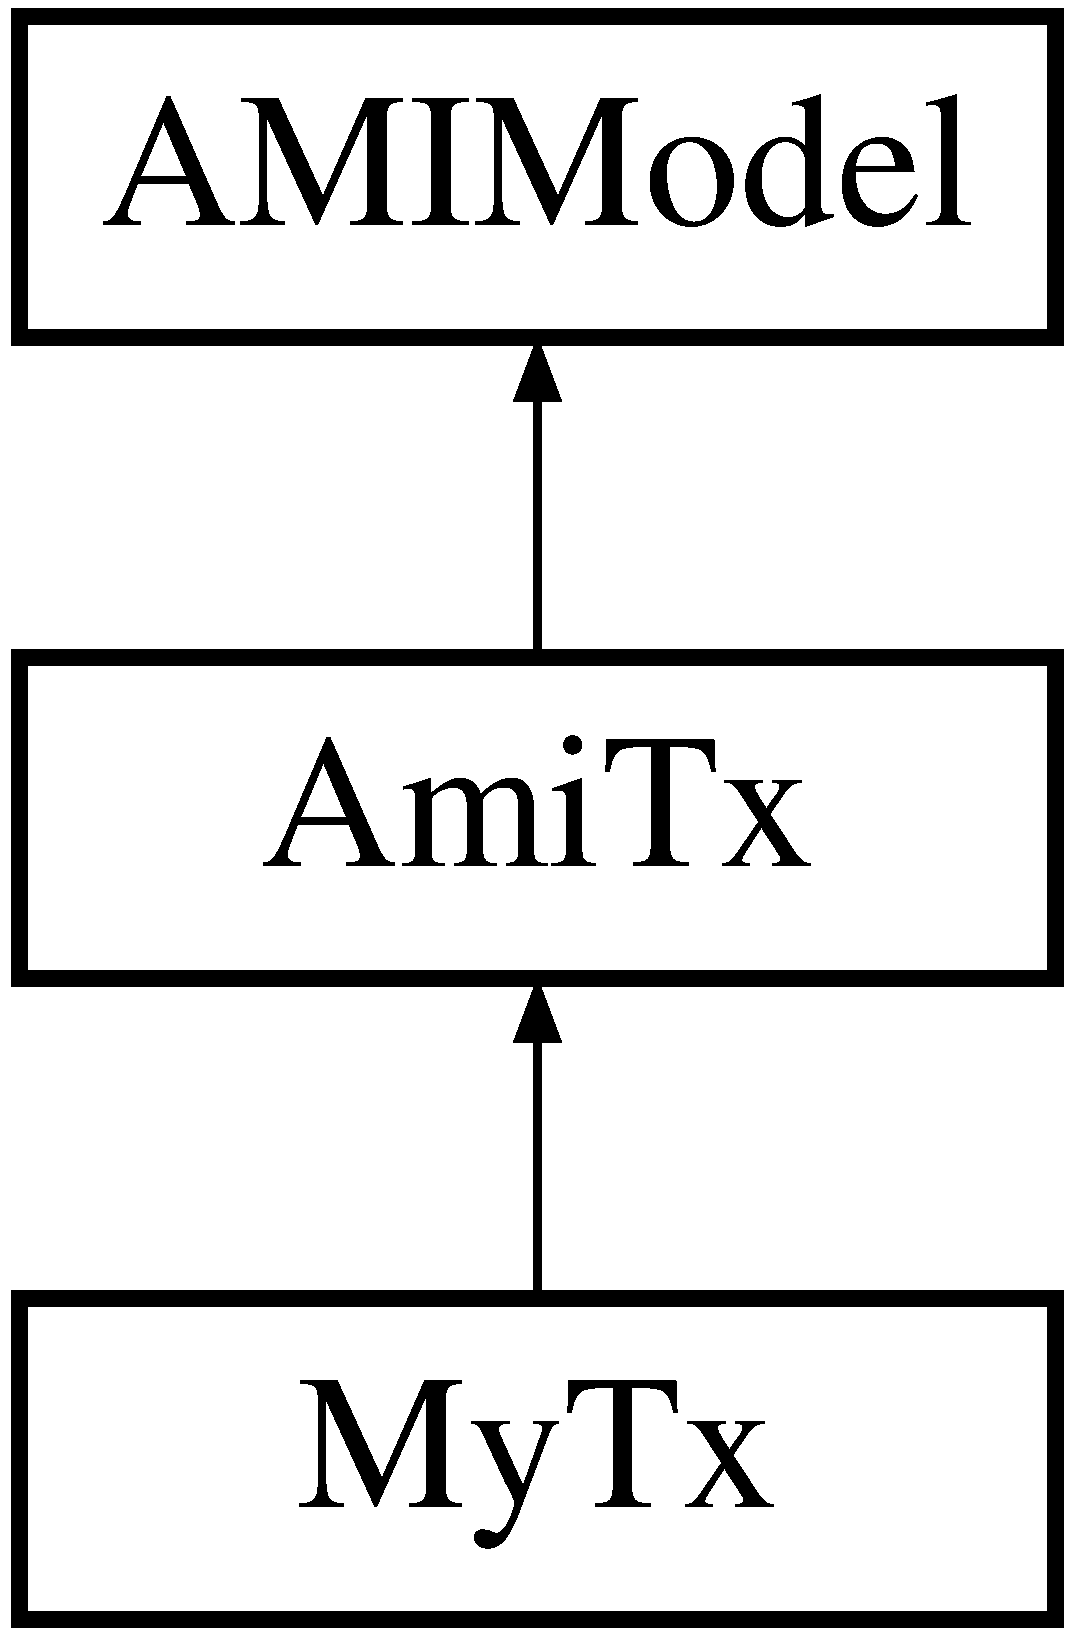
\includegraphics[height=3.000000cm]{class_a_m_i_model}
\end{center}
\end{figure}
\subsection*{Public Member Functions}
\begin{DoxyCompactItemize}
\item 
virtual \hyperlink{class_a_m_i_model_a6c266bc8306cef0ed802c49c8847e8fc}{$\sim$\+A\+M\+I\+Model} ()
\item 
virtual void \hyperlink{class_a_m_i_model_a8f45652e216686d0efa8db7e9dc0e915}{init} (double $\ast$impulse\+\_\+matrix, const long number\+\_\+of\+\_\+rows, const long aggressors, const double sample\+\_\+interval, const double bit\+\_\+time, const std\+::string \&A\+M\+I\+\_\+parameters\+\_\+in)
\begin{DoxyCompactList}\small\item\em Initialize the model. \end{DoxyCompactList}\item 
virtual void \hyperlink{class_a_m_i_model_a52d1f23607e7f12fa1ab61d809231c11}{proc\+\_\+imp} ()=0
\begin{DoxyCompactList}\small\item\em Process the incoming impulse response. \end{DoxyCompactList}\item 
std\+::string \& \hyperlink{class_a_m_i_model_ae65d47400fd3736682c229dab31392ad}{msg} ()
\begin{DoxyCompactList}\small\item\em Retrieve the model message. \end{DoxyCompactList}\item 
std\+::string \& \hyperlink{class_a_m_i_model_abb8b57f839746e955774d7bc8f1b5d02}{param\+\_\+str} ()
\begin{DoxyCompactList}\small\item\em Retrieve the model parameter string. \end{DoxyCompactList}\end{DoxyCompactItemize}
\subsection*{Protected Member Functions}
\begin{DoxyCompactItemize}
\item 
\hyperlink{amimodel_8h_a5fbe8bcd249e7070ded2dadafa23ec1f}{Parse\+Res} \hyperlink{class_a_m_i_model_ad99c8cb946fe1d0b2197253130969368}{parse\+\_\+params} (const std\+::string \&A\+M\+I\+\_\+parameters\+\_\+in)
\begin{DoxyCompactList}\small\item\em Parse the incoming A\+M\+I parameter string. \end{DoxyCompactList}\item 
std\+::string \hyperlink{class_a_m_i_model_a62437e97ce61c76f4b9af78144385416}{get\+\_\+param} (const std\+::vector$<$ std\+::string $>$ \&node\+\_\+names) const 
\begin{DoxyCompactList}\small\item\em Get the string value of a parameter. \end{DoxyCompactList}\item 
long \hyperlink{class_a_m_i_model_a55b68d8a68be34f672d53968484225e1}{get\+\_\+param\+\_\+int} (const std\+::vector$<$ std\+::string $>$ \&node\+\_\+names, long default\+\_\+val) const 
\begin{DoxyCompactList}\small\item\em Get the value of an integer parameter. \end{DoxyCompactList}\item 
void \hyperlink{class_a_m_i_model_a1e8cbd58a09b712dcf76a12f439bce30}{log} (std\+::string \hyperlink{class_a_m_i_model_ae65d47400fd3736682c229dab31392ad}{msg})
\end{DoxyCompactItemize}
\subsection*{Protected Attributes}
\begin{DoxyCompactItemize}
\item 
std\+::string \hyperlink{class_a_m_i_model_acc9d4703088b0a69f649c84a1e134cfd}{msg\+\_\+}
\item 
std\+::string \hyperlink{class_a_m_i_model_ab7aeef08245acc654271341cdf0139f9}{param\+\_\+str\+\_\+}
\item 
std\+::string \hyperlink{class_a_m_i_model_a42e00992da9baf93d81d1d9fcd32d8e6}{name\+\_\+}
\item 
double \hyperlink{class_a_m_i_model_a4d4c286b04668c22f2e3f315715a6d5b}{sample\+\_\+interval\+\_\+}
\item 
double \hyperlink{class_a_m_i_model_ad0b6751b3b3a69fb8951fde0fcdf4f27}{bit\+\_\+time\+\_\+}
\item 
double $\ast$ \hyperlink{class_a_m_i_model_a26c35bff12c048655bdbd8663a2f0f58}{impulse\+\_\+matrix\+\_\+}
\item 
long \hyperlink{class_a_m_i_model_aaaf94b76a519e60318e1874bb190e9a8}{number\+\_\+of\+\_\+rows\+\_\+}
\item 
long \hyperlink{class_a_m_i_model_aab3a042b2459b4b838cb61bf92a50d03}{aggressors\+\_\+}
\item 
\hyperlink{structibisami_1_1_param_tree}{ibisami\+::\+Param\+Tree} \hyperlink{class_a_m_i_model_a4da53456e13a1224f2bb47396ab0ecbd}{param\+\_\+tree\+\_\+}
\item 
std\+::ofstream \hyperlink{class_a_m_i_model_a9b1c44767e4e81c4dfcff9bc23907b6c}{clog\+\_\+}
\item 
bool \hyperlink{class_a_m_i_model_ae701c08f6c4b0d962df4a2f2dcb6196b}{log\+\_\+}
\end{DoxyCompactItemize}


\subsection{Detailed Description}
Abstract class providing the base functionality required by all I\+B\+I\+S-\/\+A\+M\+I models. 

Definition at line 119 of file amimodel.\+h.



\subsection{Constructor \& Destructor Documentation}
\hypertarget{class_a_m_i_model_a6c266bc8306cef0ed802c49c8847e8fc}{}\index{A\+M\+I\+Model@{A\+M\+I\+Model}!````~A\+M\+I\+Model@{$\sim$\+A\+M\+I\+Model}}
\index{````~A\+M\+I\+Model@{$\sim$\+A\+M\+I\+Model}!A\+M\+I\+Model@{A\+M\+I\+Model}}
\subsubsection[{$\sim$\+A\+M\+I\+Model}]{\setlength{\rightskip}{0pt plus 5cm}virtual A\+M\+I\+Model\+::$\sim$\+A\+M\+I\+Model (
\begin{DoxyParamCaption}
{}
\end{DoxyParamCaption}
)\hspace{0.3cm}{\ttfamily [inline]}, {\ttfamily [virtual]}}\label{class_a_m_i_model_a6c266bc8306cef0ed802c49c8847e8fc}


Definition at line 121 of file amimodel.\+h.



\subsection{Member Function Documentation}
\hypertarget{class_a_m_i_model_a62437e97ce61c76f4b9af78144385416}{}\index{A\+M\+I\+Model@{A\+M\+I\+Model}!get\+\_\+param@{get\+\_\+param}}
\index{get\+\_\+param@{get\+\_\+param}!A\+M\+I\+Model@{A\+M\+I\+Model}}
\subsubsection[{get\+\_\+param}]{\setlength{\rightskip}{0pt plus 5cm}std\+::string A\+M\+I\+Model\+::get\+\_\+param (
\begin{DoxyParamCaption}
\item[{const std\+::vector$<$ std\+::string $>$ \&}]{node\+\_\+names}
\end{DoxyParamCaption}
) const\hspace{0.3cm}{\ttfamily [protected]}}\label{class_a_m_i_model_a62437e97ce61c76f4b9af78144385416}


Get the string value of a parameter. 

Returns the string value of a particular A\+M\+I parameter.

Inputs\+:
\begin{DoxyItemize}
\item node\+\_\+names\+: A vector of strings containing the A\+M\+I parameter tree node names required to traverse our way to the parameter of interest. The root name should not be included.
\end{DoxyItemize}

Returns\+:
\begin{DoxyItemize}
\item the requested parameter\textquotesingle{}s value string, if the parameter was found.
\item empty string, otherwise. 
\end{DoxyItemize}

Definition at line 96 of file amimodel.\+cpp.

\hypertarget{class_a_m_i_model_a55b68d8a68be34f672d53968484225e1}{}\index{A\+M\+I\+Model@{A\+M\+I\+Model}!get\+\_\+param\+\_\+int@{get\+\_\+param\+\_\+int}}
\index{get\+\_\+param\+\_\+int@{get\+\_\+param\+\_\+int}!A\+M\+I\+Model@{A\+M\+I\+Model}}
\subsubsection[{get\+\_\+param\+\_\+int}]{\setlength{\rightskip}{0pt plus 5cm}long A\+M\+I\+Model\+::get\+\_\+param\+\_\+int (
\begin{DoxyParamCaption}
\item[{const std\+::vector$<$ std\+::string $>$ \&}]{node\+\_\+names, }
\item[{long}]{default\+\_\+val}
\end{DoxyParamCaption}
) const\hspace{0.3cm}{\ttfamily [protected]}}\label{class_a_m_i_model_a55b68d8a68be34f672d53968484225e1}


Get the value of an integer parameter. 

Returns the integer value of a particular Integer parameter.

Inputs\+:
\begin{DoxyItemize}
\item node\+\_\+names\+: A vector of strings containing the A\+M\+I parameter tree node names required to traverse our way to the parameter of interest. The root name should not be included.
\item default\+\_\+val\+: The value to return, if the parameter is not found in the tree.
\end{DoxyItemize}

Returns\+:
\begin{DoxyItemize}
\item the requested parameter\textquotesingle{}s integer value, if the parameter was found and an integer was able to be scanned from its value string.
\item \textquotesingle{}default\+\_\+val\textquotesingle{}, if the parameter was not found in the tree.
\end{DoxyItemize}

Throws\+:
\begin{DoxyItemize}
\item std\+::runtime\+\_\+error, if the parameter was found and an integer could not be scanned from its value string. 
\end{DoxyItemize}

Definition at line 64 of file amimodel.\+cpp.

\hypertarget{class_a_m_i_model_a8f45652e216686d0efa8db7e9dc0e915}{}\index{A\+M\+I\+Model@{A\+M\+I\+Model}!init@{init}}
\index{init@{init}!A\+M\+I\+Model@{A\+M\+I\+Model}}
\subsubsection[{init}]{\setlength{\rightskip}{0pt plus 5cm}void A\+M\+I\+Model\+::init (
\begin{DoxyParamCaption}
\item[{double $\ast$}]{impulse\+\_\+matrix, }
\item[{const long}]{number\+\_\+of\+\_\+rows, }
\item[{const long}]{aggressors, }
\item[{const double}]{sample\+\_\+interval, }
\item[{const double}]{bit\+\_\+time, }
\item[{const std\+::string \&}]{A\+M\+I\+\_\+parameters\+\_\+in}
\end{DoxyParamCaption}
)\hspace{0.3cm}{\ttfamily [virtual]}}\label{class_a_m_i_model_a8f45652e216686d0efa8db7e9dc0e915}


Initialize the model. 



Reimplemented in \hyperlink{class_my_tx_a4166bdab63c2366409998b2e606f55d2}{My\+Tx}.



Definition at line 16 of file amimodel.\+cpp.

\hypertarget{class_a_m_i_model_a1e8cbd58a09b712dcf76a12f439bce30}{}\index{A\+M\+I\+Model@{A\+M\+I\+Model}!log@{log}}
\index{log@{log}!A\+M\+I\+Model@{A\+M\+I\+Model}}
\subsubsection[{log}]{\setlength{\rightskip}{0pt plus 5cm}void A\+M\+I\+Model\+::log (
\begin{DoxyParamCaption}
\item[{std\+::string}]{msg}
\end{DoxyParamCaption}
)\hspace{0.3cm}{\ttfamily [inline]}, {\ttfamily [protected]}}\label{class_a_m_i_model_a1e8cbd58a09b712dcf76a12f439bce30}


Definition at line 133 of file amimodel.\+h.

\hypertarget{class_a_m_i_model_ae65d47400fd3736682c229dab31392ad}{}\index{A\+M\+I\+Model@{A\+M\+I\+Model}!msg@{msg}}
\index{msg@{msg}!A\+M\+I\+Model@{A\+M\+I\+Model}}
\subsubsection[{msg}]{\setlength{\rightskip}{0pt plus 5cm}std\+::string\& A\+M\+I\+Model\+::msg (
\begin{DoxyParamCaption}
{}
\end{DoxyParamCaption}
)\hspace{0.3cm}{\ttfamily [inline]}}\label{class_a_m_i_model_ae65d47400fd3736682c229dab31392ad}


Retrieve the model message. 



Definition at line 126 of file amimodel.\+h.

\hypertarget{class_a_m_i_model_abb8b57f839746e955774d7bc8f1b5d02}{}\index{A\+M\+I\+Model@{A\+M\+I\+Model}!param\+\_\+str@{param\+\_\+str}}
\index{param\+\_\+str@{param\+\_\+str}!A\+M\+I\+Model@{A\+M\+I\+Model}}
\subsubsection[{param\+\_\+str}]{\setlength{\rightskip}{0pt plus 5cm}std\+::string\& A\+M\+I\+Model\+::param\+\_\+str (
\begin{DoxyParamCaption}
{}
\end{DoxyParamCaption}
)\hspace{0.3cm}{\ttfamily [inline]}}\label{class_a_m_i_model_abb8b57f839746e955774d7bc8f1b5d02}


Retrieve the model parameter string. 



Definition at line 127 of file amimodel.\+h.

\hypertarget{class_a_m_i_model_ad99c8cb946fe1d0b2197253130969368}{}\index{A\+M\+I\+Model@{A\+M\+I\+Model}!parse\+\_\+params@{parse\+\_\+params}}
\index{parse\+\_\+params@{parse\+\_\+params}!A\+M\+I\+Model@{A\+M\+I\+Model}}
\subsubsection[{parse\+\_\+params}]{\setlength{\rightskip}{0pt plus 5cm}{\bf Parse\+Res} A\+M\+I\+Model\+::parse\+\_\+params (
\begin{DoxyParamCaption}
\item[{const std\+::string \&}]{A\+M\+I\+\_\+parameters\+\_\+in}
\end{DoxyParamCaption}
)\hspace{0.3cm}{\ttfamily [protected]}}\label{class_a_m_i_model_ad99c8cb946fe1d0b2197253130969368}


Parse the incoming A\+M\+I parameter string. 



Definition at line 30 of file amimodel.\+cpp.

\hypertarget{class_a_m_i_model_a52d1f23607e7f12fa1ab61d809231c11}{}\index{A\+M\+I\+Model@{A\+M\+I\+Model}!proc\+\_\+imp@{proc\+\_\+imp}}
\index{proc\+\_\+imp@{proc\+\_\+imp}!A\+M\+I\+Model@{A\+M\+I\+Model}}
\subsubsection[{proc\+\_\+imp}]{\setlength{\rightskip}{0pt plus 5cm}virtual void A\+M\+I\+Model\+::proc\+\_\+imp (
\begin{DoxyParamCaption}
{}
\end{DoxyParamCaption}
)\hspace{0.3cm}{\ttfamily [pure virtual]}}\label{class_a_m_i_model_a52d1f23607e7f12fa1ab61d809231c11}


Process the incoming impulse response. 



Implemented in \hyperlink{class_ami_tx_a94649674c8e8442c1d5434d509165594}{Ami\+Tx}.



\subsection{Member Data Documentation}
\hypertarget{class_a_m_i_model_aab3a042b2459b4b838cb61bf92a50d03}{}\index{A\+M\+I\+Model@{A\+M\+I\+Model}!aggressors\+\_\+@{aggressors\+\_\+}}
\index{aggressors\+\_\+@{aggressors\+\_\+}!A\+M\+I\+Model@{A\+M\+I\+Model}}
\subsubsection[{aggressors\+\_\+}]{\setlength{\rightskip}{0pt plus 5cm}long A\+M\+I\+Model\+::aggressors\+\_\+\hspace{0.3cm}{\ttfamily [protected]}}\label{class_a_m_i_model_aab3a042b2459b4b838cb61bf92a50d03}


Definition at line 137 of file amimodel.\+h.

\hypertarget{class_a_m_i_model_ad0b6751b3b3a69fb8951fde0fcdf4f27}{}\index{A\+M\+I\+Model@{A\+M\+I\+Model}!bit\+\_\+time\+\_\+@{bit\+\_\+time\+\_\+}}
\index{bit\+\_\+time\+\_\+@{bit\+\_\+time\+\_\+}!A\+M\+I\+Model@{A\+M\+I\+Model}}
\subsubsection[{bit\+\_\+time\+\_\+}]{\setlength{\rightskip}{0pt plus 5cm}double A\+M\+I\+Model\+::bit\+\_\+time\+\_\+\hspace{0.3cm}{\ttfamily [protected]}}\label{class_a_m_i_model_ad0b6751b3b3a69fb8951fde0fcdf4f27}


Definition at line 136 of file amimodel.\+h.

\hypertarget{class_a_m_i_model_a9b1c44767e4e81c4dfcff9bc23907b6c}{}\index{A\+M\+I\+Model@{A\+M\+I\+Model}!clog\+\_\+@{clog\+\_\+}}
\index{clog\+\_\+@{clog\+\_\+}!A\+M\+I\+Model@{A\+M\+I\+Model}}
\subsubsection[{clog\+\_\+}]{\setlength{\rightskip}{0pt plus 5cm}std\+::ofstream A\+M\+I\+Model\+::clog\+\_\+\hspace{0.3cm}{\ttfamily [protected]}}\label{class_a_m_i_model_a9b1c44767e4e81c4dfcff9bc23907b6c}


Definition at line 139 of file amimodel.\+h.

\hypertarget{class_a_m_i_model_a26c35bff12c048655bdbd8663a2f0f58}{}\index{A\+M\+I\+Model@{A\+M\+I\+Model}!impulse\+\_\+matrix\+\_\+@{impulse\+\_\+matrix\+\_\+}}
\index{impulse\+\_\+matrix\+\_\+@{impulse\+\_\+matrix\+\_\+}!A\+M\+I\+Model@{A\+M\+I\+Model}}
\subsubsection[{impulse\+\_\+matrix\+\_\+}]{\setlength{\rightskip}{0pt plus 5cm}double $\ast$ A\+M\+I\+Model\+::impulse\+\_\+matrix\+\_\+\hspace{0.3cm}{\ttfamily [protected]}}\label{class_a_m_i_model_a26c35bff12c048655bdbd8663a2f0f58}


Definition at line 136 of file amimodel.\+h.

\hypertarget{class_a_m_i_model_ae701c08f6c4b0d962df4a2f2dcb6196b}{}\index{A\+M\+I\+Model@{A\+M\+I\+Model}!log\+\_\+@{log\+\_\+}}
\index{log\+\_\+@{log\+\_\+}!A\+M\+I\+Model@{A\+M\+I\+Model}}
\subsubsection[{log\+\_\+}]{\setlength{\rightskip}{0pt plus 5cm}bool A\+M\+I\+Model\+::log\+\_\+\hspace{0.3cm}{\ttfamily [protected]}}\label{class_a_m_i_model_ae701c08f6c4b0d962df4a2f2dcb6196b}


Definition at line 140 of file amimodel.\+h.

\hypertarget{class_a_m_i_model_acc9d4703088b0a69f649c84a1e134cfd}{}\index{A\+M\+I\+Model@{A\+M\+I\+Model}!msg\+\_\+@{msg\+\_\+}}
\index{msg\+\_\+@{msg\+\_\+}!A\+M\+I\+Model@{A\+M\+I\+Model}}
\subsubsection[{msg\+\_\+}]{\setlength{\rightskip}{0pt plus 5cm}std\+::string A\+M\+I\+Model\+::msg\+\_\+\hspace{0.3cm}{\ttfamily [protected]}}\label{class_a_m_i_model_acc9d4703088b0a69f649c84a1e134cfd}


Definition at line 135 of file amimodel.\+h.

\hypertarget{class_a_m_i_model_a42e00992da9baf93d81d1d9fcd32d8e6}{}\index{A\+M\+I\+Model@{A\+M\+I\+Model}!name\+\_\+@{name\+\_\+}}
\index{name\+\_\+@{name\+\_\+}!A\+M\+I\+Model@{A\+M\+I\+Model}}
\subsubsection[{name\+\_\+}]{\setlength{\rightskip}{0pt plus 5cm}std\+::string A\+M\+I\+Model\+::name\+\_\+\hspace{0.3cm}{\ttfamily [protected]}}\label{class_a_m_i_model_a42e00992da9baf93d81d1d9fcd32d8e6}


Definition at line 135 of file amimodel.\+h.

\hypertarget{class_a_m_i_model_aaaf94b76a519e60318e1874bb190e9a8}{}\index{A\+M\+I\+Model@{A\+M\+I\+Model}!number\+\_\+of\+\_\+rows\+\_\+@{number\+\_\+of\+\_\+rows\+\_\+}}
\index{number\+\_\+of\+\_\+rows\+\_\+@{number\+\_\+of\+\_\+rows\+\_\+}!A\+M\+I\+Model@{A\+M\+I\+Model}}
\subsubsection[{number\+\_\+of\+\_\+rows\+\_\+}]{\setlength{\rightskip}{0pt plus 5cm}long A\+M\+I\+Model\+::number\+\_\+of\+\_\+rows\+\_\+\hspace{0.3cm}{\ttfamily [protected]}}\label{class_a_m_i_model_aaaf94b76a519e60318e1874bb190e9a8}


Definition at line 137 of file amimodel.\+h.

\hypertarget{class_a_m_i_model_ab7aeef08245acc654271341cdf0139f9}{}\index{A\+M\+I\+Model@{A\+M\+I\+Model}!param\+\_\+str\+\_\+@{param\+\_\+str\+\_\+}}
\index{param\+\_\+str\+\_\+@{param\+\_\+str\+\_\+}!A\+M\+I\+Model@{A\+M\+I\+Model}}
\subsubsection[{param\+\_\+str\+\_\+}]{\setlength{\rightskip}{0pt plus 5cm}std\+::string A\+M\+I\+Model\+::param\+\_\+str\+\_\+\hspace{0.3cm}{\ttfamily [protected]}}\label{class_a_m_i_model_ab7aeef08245acc654271341cdf0139f9}


Definition at line 135 of file amimodel.\+h.

\hypertarget{class_a_m_i_model_a4da53456e13a1224f2bb47396ab0ecbd}{}\index{A\+M\+I\+Model@{A\+M\+I\+Model}!param\+\_\+tree\+\_\+@{param\+\_\+tree\+\_\+}}
\index{param\+\_\+tree\+\_\+@{param\+\_\+tree\+\_\+}!A\+M\+I\+Model@{A\+M\+I\+Model}}
\subsubsection[{param\+\_\+tree\+\_\+}]{\setlength{\rightskip}{0pt plus 5cm}{\bf ibisami\+::\+Param\+Tree} A\+M\+I\+Model\+::param\+\_\+tree\+\_\+\hspace{0.3cm}{\ttfamily [protected]}}\label{class_a_m_i_model_a4da53456e13a1224f2bb47396ab0ecbd}


Definition at line 138 of file amimodel.\+h.

\hypertarget{class_a_m_i_model_a4d4c286b04668c22f2e3f315715a6d5b}{}\index{A\+M\+I\+Model@{A\+M\+I\+Model}!sample\+\_\+interval\+\_\+@{sample\+\_\+interval\+\_\+}}
\index{sample\+\_\+interval\+\_\+@{sample\+\_\+interval\+\_\+}!A\+M\+I\+Model@{A\+M\+I\+Model}}
\subsubsection[{sample\+\_\+interval\+\_\+}]{\setlength{\rightskip}{0pt plus 5cm}double A\+M\+I\+Model\+::sample\+\_\+interval\+\_\+\hspace{0.3cm}{\ttfamily [protected]}}\label{class_a_m_i_model_a4d4c286b04668c22f2e3f315715a6d5b}


Definition at line 136 of file amimodel.\+h.



The documentation for this class was generated from the following files\+:\begin{DoxyCompactItemize}
\item 
ibisami/include/\hyperlink{amimodel_8h}{amimodel.\+h}\item 
ibisami/src/\hyperlink{amimodel_8cpp}{amimodel.\+cpp}\end{DoxyCompactItemize}

\hypertarget{struct_ami_pointers}{}\section{Ami\+Pointers Struct Reference}
\label{struct_ami_pointers}\index{Ami\+Pointers@{Ami\+Pointers}}


Holds the pointers, which we pass back to the \hyperlink{ibisami__api_8cpp_a2518d31187e06bed6023ec23657faab9}{A\+M\+I\+\_\+\+Init()} caller.  


\subsection*{Public Attributes}
\begin{DoxyCompactItemize}
\item 
\hyperlink{class_a_m_i_model}{A\+M\+I\+Model} $\ast$ \hyperlink{struct_ami_pointers_a382ab778612377867999da1da37eb970}{model}
\item 
char $\ast$ \hyperlink{struct_ami_pointers_a4922e9e0eb86e7515c5d60a4be512657}{msg}
\item 
char $\ast$ \hyperlink{struct_ami_pointers_a4a71183d01dde25a4cb9fabb89ee6d01}{params}
\end{DoxyCompactItemize}


\subsection{Detailed Description}
Holds the pointers, which we pass back to the \hyperlink{ibisami__api_8cpp_a2518d31187e06bed6023ec23657faab9}{A\+M\+I\+\_\+\+Init()} caller. 

Definition at line 23 of file ibisami\+\_\+api.\+cpp.



\subsection{Member Data Documentation}
\hypertarget{struct_ami_pointers_a382ab778612377867999da1da37eb970}{}\index{Ami\+Pointers@{Ami\+Pointers}!model@{model}}
\index{model@{model}!Ami\+Pointers@{Ami\+Pointers}}
\subsubsection[{model}]{\setlength{\rightskip}{0pt plus 5cm}{\bf A\+M\+I\+Model}$\ast$ Ami\+Pointers\+::model}\label{struct_ami_pointers_a382ab778612377867999da1da37eb970}


Definition at line 24 of file ibisami\+\_\+api.\+cpp.

\hypertarget{struct_ami_pointers_a4922e9e0eb86e7515c5d60a4be512657}{}\index{Ami\+Pointers@{Ami\+Pointers}!msg@{msg}}
\index{msg@{msg}!Ami\+Pointers@{Ami\+Pointers}}
\subsubsection[{msg}]{\setlength{\rightskip}{0pt plus 5cm}char$\ast$ Ami\+Pointers\+::msg}\label{struct_ami_pointers_a4922e9e0eb86e7515c5d60a4be512657}


Definition at line 25 of file ibisami\+\_\+api.\+cpp.

\hypertarget{struct_ami_pointers_a4a71183d01dde25a4cb9fabb89ee6d01}{}\index{Ami\+Pointers@{Ami\+Pointers}!params@{params}}
\index{params@{params}!Ami\+Pointers@{Ami\+Pointers}}
\subsubsection[{params}]{\setlength{\rightskip}{0pt plus 5cm}char$\ast$ Ami\+Pointers\+::params}\label{struct_ami_pointers_a4a71183d01dde25a4cb9fabb89ee6d01}


Definition at line 26 of file ibisami\+\_\+api.\+cpp.



The documentation for this struct was generated from the following file\+:\begin{DoxyCompactItemize}
\item 
src/\hyperlink{ibisami__api_8cpp}{ibisami\+\_\+api.\+cpp}\end{DoxyCompactItemize}

\hypertarget{class_ami_tx}{}\section{Ami\+Tx Class Reference}
\label{class_ami_tx}\index{Ami\+Tx@{Ami\+Tx}}


A generic I\+B\+I\+S-\/\+A\+M\+I Tx model implementation.  




{\ttfamily \#include $<$ami\+\_\+tx.\+h$>$}

Inheritance diagram for Ami\+Tx\+:\begin{figure}[H]
\begin{center}
\leavevmode
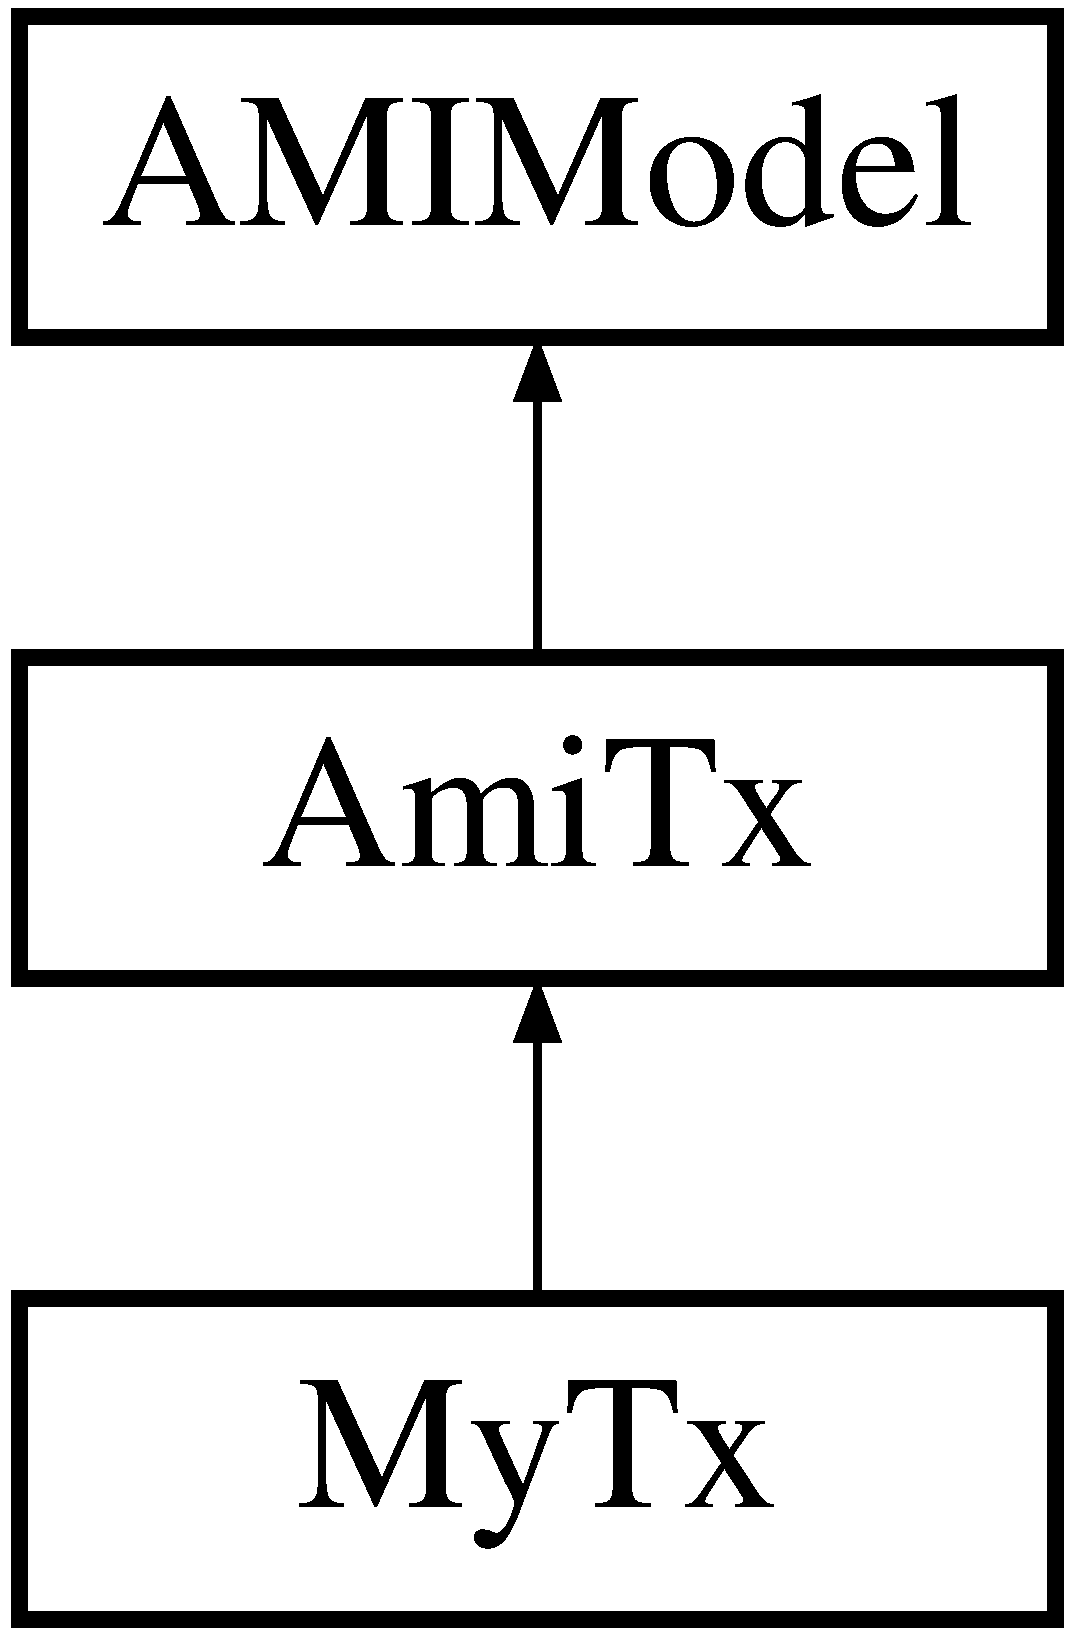
\includegraphics[height=3.000000cm]{class_ami_tx}
\end{center}
\end{figure}
\subsection*{Public Member Functions}
\begin{DoxyCompactItemize}
\item 
virtual \hyperlink{class_ami_tx_a0a30ee85116e1f2ba7c4a8876c0b7b8e}{$\sim$\+Ami\+Tx} ()
\item 
void \hyperlink{class_ami_tx_a94649674c8e8442c1d5434d509165594}{proc\+\_\+imp} () override
\begin{DoxyCompactList}\small\item\em Process the channel impulse response. \end{DoxyCompactList}\item 
bool \hyperlink{class_ami_tx_a8f326f6dfa875c00800491ff2104f248}{proc\+\_\+sig} (double $\ast$sig, long len, double $\ast$clock\+\_\+times) override
\begin{DoxyCompactList}\small\item\em Process a signal. \end{DoxyCompactList}\end{DoxyCompactItemize}
\subsection*{Protected Attributes}
\begin{DoxyCompactItemize}
\item 
\hyperlink{class_digital_filter}{Digital\+Filter} $\ast$ \hyperlink{class_ami_tx_a1eb407f2a0aa1010c5d381c172f8425d}{filter\+\_\+}
\begin{DoxyCompactList}\small\item\em Used for pre-\/emphasis. \end{DoxyCompactList}\item 
bool \hyperlink{class_ami_tx_a8e07817524a3626aaa432bcbe7cad30f}{have\+\_\+preemph\+\_\+}
\begin{DoxyCompactList}\small\item\em True, if I have a pre-\/emphasis filter. \end{DoxyCompactList}\item 
int \hyperlink{class_ami_tx_a166891685483a94632bbcd4e2afebf88}{num\+\_\+taps\+\_\+}
\begin{DoxyCompactList}\small\item\em Number of taps in my pre-\/emphasis filter. \end{DoxyCompactList}\item 
std\+::vector$<$ double $>$ \hyperlink{class_ami_tx_ab4878fcf087a793ca120ab1e30cabed5}{tap\+\_\+weights\+\_\+}
\begin{DoxyCompactList}\small\item\em Tap weights for pre-\/emphasis filter. \end{DoxyCompactList}\end{DoxyCompactItemize}
\subsection*{Additional Inherited Members}


\subsection{Detailed Description}
A generic I\+B\+I\+S-\/\+A\+M\+I Tx model implementation. 

This abstract class provides generic Tx model capability. Device specific Tx models should derive from this class. 

Definition at line 23 of file ami\+\_\+tx.\+h.



\subsection{Constructor \& Destructor Documentation}
\hypertarget{class_ami_tx_a0a30ee85116e1f2ba7c4a8876c0b7b8e}{}\index{Ami\+Tx@{Ami\+Tx}!````~Ami\+Tx@{$\sim$\+Ami\+Tx}}
\index{````~Ami\+Tx@{$\sim$\+Ami\+Tx}!Ami\+Tx@{Ami\+Tx}}
\subsubsection[{$\sim$\+Ami\+Tx}]{\setlength{\rightskip}{0pt plus 5cm}virtual Ami\+Tx\+::$\sim$\+Ami\+Tx (
\begin{DoxyParamCaption}
{}
\end{DoxyParamCaption}
)\hspace{0.3cm}{\ttfamily [inline]}, {\ttfamily [virtual]}}\label{class_ami_tx_a0a30ee85116e1f2ba7c4a8876c0b7b8e}


Definition at line 26 of file ami\+\_\+tx.\+h.



\subsection{Member Function Documentation}
\hypertarget{class_ami_tx_a94649674c8e8442c1d5434d509165594}{}\index{Ami\+Tx@{Ami\+Tx}!proc\+\_\+imp@{proc\+\_\+imp}}
\index{proc\+\_\+imp@{proc\+\_\+imp}!Ami\+Tx@{Ami\+Tx}}
\subsubsection[{proc\+\_\+imp}]{\setlength{\rightskip}{0pt plus 5cm}void Ami\+Tx\+::proc\+\_\+imp (
\begin{DoxyParamCaption}
{}
\end{DoxyParamCaption}
)\hspace{0.3cm}{\ttfamily [override]}, {\ttfamily [virtual]}}\label{class_ami_tx_a94649674c8e8442c1d5434d509165594}


Process the channel impulse response. 



Implements \hyperlink{class_a_m_i_model_a52d1f23607e7f12fa1ab61d809231c11}{A\+M\+I\+Model}.



Definition at line 14 of file ami\+\_\+tx.\+cpp.

\hypertarget{class_ami_tx_a8f326f6dfa875c00800491ff2104f248}{}\index{Ami\+Tx@{Ami\+Tx}!proc\+\_\+sig@{proc\+\_\+sig}}
\index{proc\+\_\+sig@{proc\+\_\+sig}!Ami\+Tx@{Ami\+Tx}}
\subsubsection[{proc\+\_\+sig}]{\setlength{\rightskip}{0pt plus 5cm}bool Ami\+Tx\+::proc\+\_\+sig (
\begin{DoxyParamCaption}
\item[{double $\ast$}]{sig, }
\item[{long}]{len, }
\item[{double $\ast$}]{clock\+\_\+times}
\end{DoxyParamCaption}
)\hspace{0.3cm}{\ttfamily [override]}, {\ttfamily [virtual]}}\label{class_ami_tx_a8f326f6dfa875c00800491ff2104f248}


Process a signal. 


\begin{DoxyParams}{Parameters}
{\em sig} & A pointer to the array of doubles to be processed. \\
\hline
{\em len} & The number of samples to process. \\
\hline
{\em clock\+\_\+times} & A pointer to the array of doubles used for storing the clock times. \\
\hline
\end{DoxyParams}
\begin{DoxyReturn}{Returns}
A Boolean flag, which is true if the model reached steady state, regarding any adaptation.
\end{DoxyReturn}
As per the I\+B\+I\+S standard, the user is allowed to presume that there has been enough storage allocated for clock\+\_\+times, given the value of sig\+\_\+len, sample\+\_\+interval, and bit\+\_\+time.

\begin{DoxySeeAlso}{See also}
\hyperlink{class_a_m_i_model_a8f45652e216686d0efa8db7e9dc0e915}{init()} 
\end{DoxySeeAlso}


Implements \hyperlink{class_a_m_i_model_abb1d05835230a1b0e8f6b98002d8f4ef}{A\+M\+I\+Model}.



Definition at line 30 of file ami\+\_\+tx.\+cpp.



\subsection{Member Data Documentation}
\hypertarget{class_ami_tx_a1eb407f2a0aa1010c5d381c172f8425d}{}\index{Ami\+Tx@{Ami\+Tx}!filter\+\_\+@{filter\+\_\+}}
\index{filter\+\_\+@{filter\+\_\+}!Ami\+Tx@{Ami\+Tx}}
\subsubsection[{filter\+\_\+}]{\setlength{\rightskip}{0pt plus 5cm}{\bf Digital\+Filter}$\ast$ Ami\+Tx\+::filter\+\_\+\hspace{0.3cm}{\ttfamily [protected]}}\label{class_ami_tx_a1eb407f2a0aa1010c5d381c172f8425d}


Used for pre-\/emphasis. 



Definition at line 31 of file ami\+\_\+tx.\+h.

\hypertarget{class_ami_tx_a8e07817524a3626aaa432bcbe7cad30f}{}\index{Ami\+Tx@{Ami\+Tx}!have\+\_\+preemph\+\_\+@{have\+\_\+preemph\+\_\+}}
\index{have\+\_\+preemph\+\_\+@{have\+\_\+preemph\+\_\+}!Ami\+Tx@{Ami\+Tx}}
\subsubsection[{have\+\_\+preemph\+\_\+}]{\setlength{\rightskip}{0pt plus 5cm}bool Ami\+Tx\+::have\+\_\+preemph\+\_\+\hspace{0.3cm}{\ttfamily [protected]}}\label{class_ami_tx_a8e07817524a3626aaa432bcbe7cad30f}


True, if I have a pre-\/emphasis filter. 



Definition at line 32 of file ami\+\_\+tx.\+h.

\hypertarget{class_ami_tx_a166891685483a94632bbcd4e2afebf88}{}\index{Ami\+Tx@{Ami\+Tx}!num\+\_\+taps\+\_\+@{num\+\_\+taps\+\_\+}}
\index{num\+\_\+taps\+\_\+@{num\+\_\+taps\+\_\+}!Ami\+Tx@{Ami\+Tx}}
\subsubsection[{num\+\_\+taps\+\_\+}]{\setlength{\rightskip}{0pt plus 5cm}int Ami\+Tx\+::num\+\_\+taps\+\_\+\hspace{0.3cm}{\ttfamily [protected]}}\label{class_ami_tx_a166891685483a94632bbcd4e2afebf88}


Number of taps in my pre-\/emphasis filter. 



Definition at line 33 of file ami\+\_\+tx.\+h.

\hypertarget{class_ami_tx_ab4878fcf087a793ca120ab1e30cabed5}{}\index{Ami\+Tx@{Ami\+Tx}!tap\+\_\+weights\+\_\+@{tap\+\_\+weights\+\_\+}}
\index{tap\+\_\+weights\+\_\+@{tap\+\_\+weights\+\_\+}!Ami\+Tx@{Ami\+Tx}}
\subsubsection[{tap\+\_\+weights\+\_\+}]{\setlength{\rightskip}{0pt plus 5cm}std\+::vector$<$double$>$ Ami\+Tx\+::tap\+\_\+weights\+\_\+\hspace{0.3cm}{\ttfamily [protected]}}\label{class_ami_tx_ab4878fcf087a793ca120ab1e30cabed5}


Tap weights for pre-\/emphasis filter. 



Definition at line 34 of file ami\+\_\+tx.\+h.



The documentation for this class was generated from the following files\+:\begin{DoxyCompactItemize}
\item 
include/\hyperlink{ami__tx_8h}{ami\+\_\+tx.\+h}\item 
src/\hyperlink{ami__tx_8cpp}{ami\+\_\+tx.\+cpp}\end{DoxyCompactItemize}

\hypertarget{class_digital_filter}{}\section{Digital\+Filter Class Reference}
\label{class_digital_filter}\index{Digital\+Filter@{Digital\+Filter}}


A generic digital filter implementation, using \char`\"{}\+Direct Form 2\char`\"{} processing.  




{\ttfamily \#include $<$digital\+\_\+filter.\+h$>$}

\subsection*{Public Member Functions}
\begin{DoxyCompactItemize}
\item 
\hyperlink{class_digital_filter_aa3d504c14a3dd71c0a8384e03fb9a3b8}{Digital\+Filter} (const std\+::vector$<$ double $>$ \&num, const std\+::vector$<$ double $>$ \&den)
\begin{DoxyCompactList}\small\item\em Constructor. \end{DoxyCompactList}\item 
virtual \hyperlink{class_digital_filter_a6d4f521ddcfaa2bfabc302cb590cc9e1}{$\sim$\+Digital\+Filter} ()
\item 
void \hyperlink{class_digital_filter_ab9e95357beb9cca85546dfa6714a0fb2}{apply} (double $\ast$sig, const long len)
\begin{DoxyCompactList}\small\item\em Filter application. \end{DoxyCompactList}\end{DoxyCompactItemize}
\subsection*{Protected Attributes}
\begin{DoxyCompactItemize}
\item 
std\+::vector$<$ double $>$ \hyperlink{class_digital_filter_abf0263de2d7837bdc002615d3d7ca365}{num\+\_\+}
\item 
std\+::vector$<$ double $>$ \hyperlink{class_digital_filter_aff805e69237ae6c450221f0d4c253bf9}{den\+\_\+}
\item 
std\+::vector$<$ double $>$ \hyperlink{class_digital_filter_a0fe7f91edef50acb1d8fb68957b71129}{state\+\_\+}
\item 
int \hyperlink{class_digital_filter_ad9099f4f1da3f23988591b9e733861d7}{num\+\_\+taps\+\_\+}
\end{DoxyCompactItemize}


\subsection{Detailed Description}
A generic digital filter implementation, using \char`\"{}\+Direct Form 2\char`\"{} processing. 

Definition at line 18 of file digital\+\_\+filter.\+h.



\subsection{Constructor \& Destructor Documentation}
\hypertarget{class_digital_filter_aa3d504c14a3dd71c0a8384e03fb9a3b8}{}\index{Digital\+Filter@{Digital\+Filter}!Digital\+Filter@{Digital\+Filter}}
\index{Digital\+Filter@{Digital\+Filter}!Digital\+Filter@{Digital\+Filter}}
\subsubsection[{Digital\+Filter}]{\setlength{\rightskip}{0pt plus 5cm}Digital\+Filter\+::\+Digital\+Filter (
\begin{DoxyParamCaption}
\item[{const std\+::vector$<$ double $>$ \&}]{num, }
\item[{const std\+::vector$<$ double $>$ \&}]{den}
\end{DoxyParamCaption}
)}\label{class_digital_filter_aa3d504c14a3dd71c0a8384e03fb9a3b8}


Constructor. 


\begin{DoxyParams}{Parameters}
{\em num} & A vector of doubles forming the numerator of the filter response. \\
\hline
{\em den} & A vector of doubles forming the denominator of the filter response. \\
\hline
\end{DoxyParams}


Definition at line 18 of file digital\+\_\+filter.\+cpp.

\hypertarget{class_digital_filter_a6d4f521ddcfaa2bfabc302cb590cc9e1}{}\index{Digital\+Filter@{Digital\+Filter}!````~Digital\+Filter@{$\sim$\+Digital\+Filter}}
\index{````~Digital\+Filter@{$\sim$\+Digital\+Filter}!Digital\+Filter@{Digital\+Filter}}
\subsubsection[{$\sim$\+Digital\+Filter}]{\setlength{\rightskip}{0pt plus 5cm}virtual Digital\+Filter\+::$\sim$\+Digital\+Filter (
\begin{DoxyParamCaption}
{}
\end{DoxyParamCaption}
)\hspace{0.3cm}{\ttfamily [inline]}, {\ttfamily [virtual]}}\label{class_digital_filter_a6d4f521ddcfaa2bfabc302cb590cc9e1}


Definition at line 22 of file digital\+\_\+filter.\+h.



\subsection{Member Function Documentation}
\hypertarget{class_digital_filter_ab9e95357beb9cca85546dfa6714a0fb2}{}\index{Digital\+Filter@{Digital\+Filter}!apply@{apply}}
\index{apply@{apply}!Digital\+Filter@{Digital\+Filter}}
\subsubsection[{apply}]{\setlength{\rightskip}{0pt plus 5cm}void Digital\+Filter\+::apply (
\begin{DoxyParamCaption}
\item[{double $\ast$}]{sig, }
\item[{const long}]{len}
\end{DoxyParamCaption}
)}\label{class_digital_filter_ab9e95357beb9cca85546dfa6714a0fb2}


Filter application. 


\begin{DoxyParams}{Parameters}
{\em sig} & A pointer to the vector of doubles to be processed. \\
\hline
{\em len} & The number of samples to process. \\
\hline
\end{DoxyParams}


Definition at line 49 of file digital\+\_\+filter.\+cpp.



\subsection{Member Data Documentation}
\hypertarget{class_digital_filter_aff805e69237ae6c450221f0d4c253bf9}{}\index{Digital\+Filter@{Digital\+Filter}!den\+\_\+@{den\+\_\+}}
\index{den\+\_\+@{den\+\_\+}!Digital\+Filter@{Digital\+Filter}}
\subsubsection[{den\+\_\+}]{\setlength{\rightskip}{0pt plus 5cm}std\+::vector$<$double$>$ Digital\+Filter\+::den\+\_\+\hspace{0.3cm}{\ttfamily [protected]}}\label{class_digital_filter_aff805e69237ae6c450221f0d4c253bf9}


Definition at line 26 of file digital\+\_\+filter.\+h.

\hypertarget{class_digital_filter_abf0263de2d7837bdc002615d3d7ca365}{}\index{Digital\+Filter@{Digital\+Filter}!num\+\_\+@{num\+\_\+}}
\index{num\+\_\+@{num\+\_\+}!Digital\+Filter@{Digital\+Filter}}
\subsubsection[{num\+\_\+}]{\setlength{\rightskip}{0pt plus 5cm}std\+::vector$<$double$>$ Digital\+Filter\+::num\+\_\+\hspace{0.3cm}{\ttfamily [protected]}}\label{class_digital_filter_abf0263de2d7837bdc002615d3d7ca365}


Definition at line 26 of file digital\+\_\+filter.\+h.

\hypertarget{class_digital_filter_ad9099f4f1da3f23988591b9e733861d7}{}\index{Digital\+Filter@{Digital\+Filter}!num\+\_\+taps\+\_\+@{num\+\_\+taps\+\_\+}}
\index{num\+\_\+taps\+\_\+@{num\+\_\+taps\+\_\+}!Digital\+Filter@{Digital\+Filter}}
\subsubsection[{num\+\_\+taps\+\_\+}]{\setlength{\rightskip}{0pt plus 5cm}int Digital\+Filter\+::num\+\_\+taps\+\_\+\hspace{0.3cm}{\ttfamily [protected]}}\label{class_digital_filter_ad9099f4f1da3f23988591b9e733861d7}


Definition at line 27 of file digital\+\_\+filter.\+h.

\hypertarget{class_digital_filter_a0fe7f91edef50acb1d8fb68957b71129}{}\index{Digital\+Filter@{Digital\+Filter}!state\+\_\+@{state\+\_\+}}
\index{state\+\_\+@{state\+\_\+}!Digital\+Filter@{Digital\+Filter}}
\subsubsection[{state\+\_\+}]{\setlength{\rightskip}{0pt plus 5cm}std\+::vector$<$double$>$ Digital\+Filter\+::state\+\_\+\hspace{0.3cm}{\ttfamily [protected]}}\label{class_digital_filter_a0fe7f91edef50acb1d8fb68957b71129}


Definition at line 26 of file digital\+\_\+filter.\+h.



The documentation for this class was generated from the following files\+:\begin{DoxyCompactItemize}
\item 
ibisami/include/\hyperlink{digital__filter_8h}{digital\+\_\+filter.\+h}\item 
ibisami/src/\hyperlink{digital__filter_8cpp}{digital\+\_\+filter.\+cpp}\end{DoxyCompactItemize}

\hypertarget{class_my_tx}{}\section{My\+Tx Class Reference}
\label{class_my_tx}\index{My\+Tx@{My\+Tx}}


An example device specific Tx model implementation.  


Inheritance diagram for My\+Tx\+:\begin{figure}[H]
\begin{center}
\leavevmode
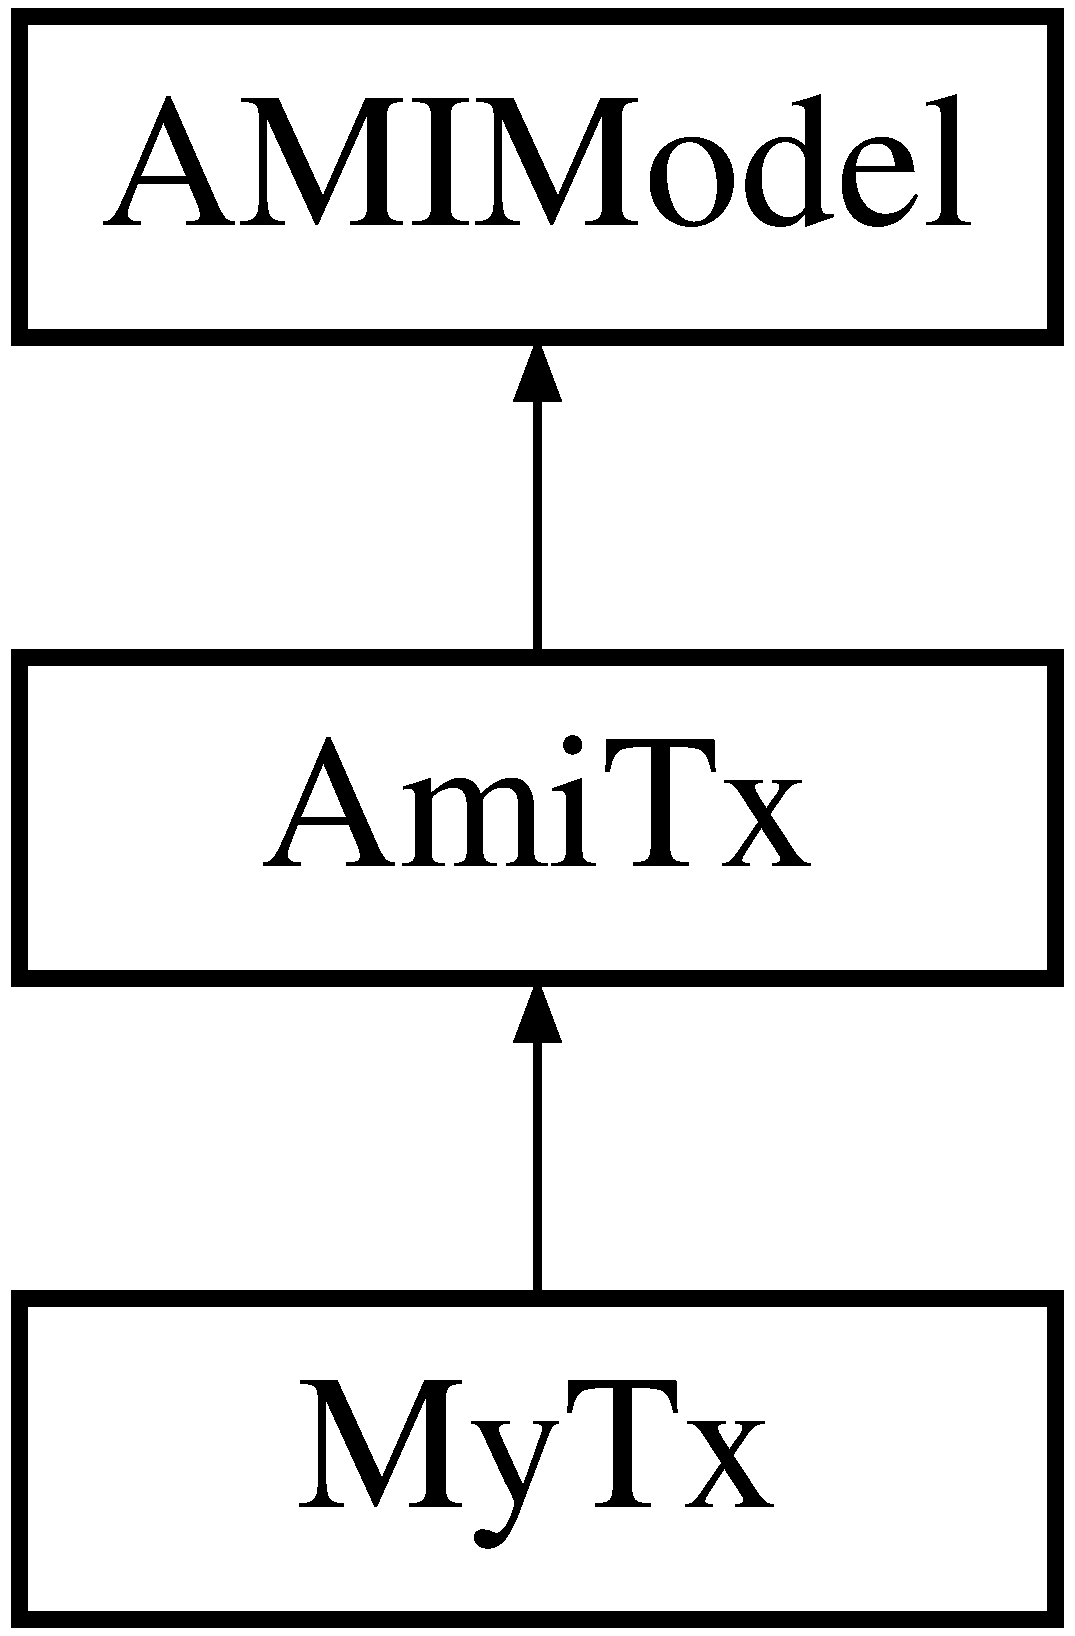
\includegraphics[height=3.000000cm]{class_my_tx}
\end{center}
\end{figure}
\subsection*{Public Member Functions}
\begin{DoxyCompactItemize}
\item 
\hyperlink{class_my_tx_a1fe85e2eeacfdc9fb6b1bf77702243be}{My\+Tx} ()
\item 
\hyperlink{class_my_tx_ab7d79dd462919d22f1ec7e33e448e0ff}{$\sim$\+My\+Tx} ()
\item 
void \hyperlink{class_my_tx_a4166bdab63c2366409998b2e606f55d2}{init} (double $\ast$impulse\+\_\+matrix, const long number\+\_\+of\+\_\+rows, const long aggressors, const double sample\+\_\+interval, const double bit\+\_\+time, const std\+::string \&A\+M\+I\+\_\+parameters\+\_\+in) override
\begin{DoxyCompactList}\small\item\em Initialize the model. \end{DoxyCompactList}\end{DoxyCompactItemize}
\subsection*{Additional Inherited Members}


\subsection{Detailed Description}
An example device specific Tx model implementation. 

Definition at line 17 of file example\+\_\+tx.\+cpp.



\subsection{Constructor \& Destructor Documentation}
\hypertarget{class_my_tx_a1fe85e2eeacfdc9fb6b1bf77702243be}{}\index{My\+Tx@{My\+Tx}!My\+Tx@{My\+Tx}}
\index{My\+Tx@{My\+Tx}!My\+Tx@{My\+Tx}}
\subsubsection[{My\+Tx}]{\setlength{\rightskip}{0pt plus 5cm}My\+Tx\+::\+My\+Tx (
\begin{DoxyParamCaption}
{}
\end{DoxyParamCaption}
)\hspace{0.3cm}{\ttfamily [inline]}}\label{class_my_tx_a1fe85e2eeacfdc9fb6b1bf77702243be}


Definition at line 21 of file example\+\_\+tx.\+cpp.

\hypertarget{class_my_tx_ab7d79dd462919d22f1ec7e33e448e0ff}{}\index{My\+Tx@{My\+Tx}!````~My\+Tx@{$\sim$\+My\+Tx}}
\index{````~My\+Tx@{$\sim$\+My\+Tx}!My\+Tx@{My\+Tx}}
\subsubsection[{$\sim$\+My\+Tx}]{\setlength{\rightskip}{0pt plus 5cm}My\+Tx\+::$\sim$\+My\+Tx (
\begin{DoxyParamCaption}
{}
\end{DoxyParamCaption}
)\hspace{0.3cm}{\ttfamily [inline]}}\label{class_my_tx_ab7d79dd462919d22f1ec7e33e448e0ff}


Definition at line 22 of file example\+\_\+tx.\+cpp.



\subsection{Member Function Documentation}
\hypertarget{class_my_tx_a4166bdab63c2366409998b2e606f55d2}{}\index{My\+Tx@{My\+Tx}!init@{init}}
\index{init@{init}!My\+Tx@{My\+Tx}}
\subsubsection[{init}]{\setlength{\rightskip}{0pt plus 5cm}void My\+Tx\+::init (
\begin{DoxyParamCaption}
\item[{double $\ast$}]{impulse\+\_\+matrix, }
\item[{const long}]{number\+\_\+of\+\_\+rows, }
\item[{const long}]{aggressors, }
\item[{const double}]{sample\+\_\+interval, }
\item[{const double}]{bit\+\_\+time, }
\item[{const std\+::string \&}]{A\+M\+I\+\_\+parameters\+\_\+in}
\end{DoxyParamCaption}
)\hspace{0.3cm}{\ttfamily [inline]}, {\ttfamily [override]}, {\ttfamily [virtual]}}\label{class_my_tx_a4166bdab63c2366409998b2e606f55d2}


Initialize the model. 



Reimplemented from \hyperlink{class_a_m_i_model_a8f45652e216686d0efa8db7e9dc0e915}{A\+M\+I\+Model}.



Definition at line 23 of file example\+\_\+tx.\+cpp.



The documentation for this class was generated from the following file\+:\begin{DoxyCompactItemize}
\item 
example/\hyperlink{example__tx_8cpp}{example\+\_\+tx.\+cpp}\end{DoxyCompactItemize}

\hypertarget{structibisami_1_1_node}{}\section{ibisami\+:\+:Node Struct Reference}
\label{structibisami_1_1_node}\index{ibisami\+::\+Node@{ibisami\+::\+Node}}


Used to access a {\itshape branch} node.  




{\ttfamily \#include $<$amimodel.\+h$>$}

Inheritance diagram for ibisami\+:\+:Node\+:\begin{figure}[H]
\begin{center}
\leavevmode
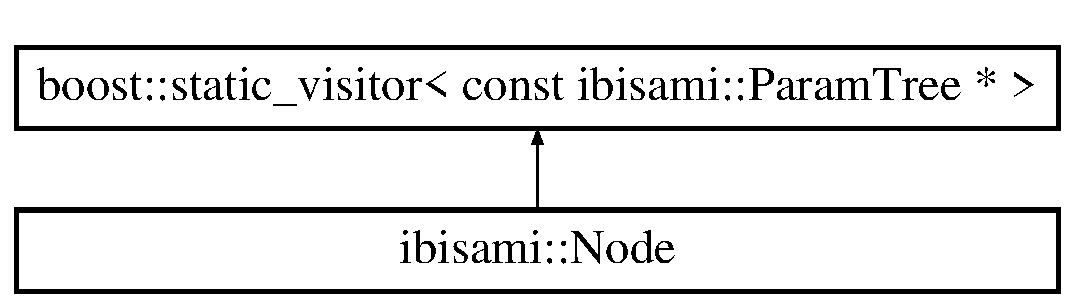
\includegraphics[height=2.000000cm]{structibisami_1_1_node}
\end{center}
\end{figure}
\subsection*{Public Member Functions}
\begin{DoxyCompactItemize}
\item 
const \hyperlink{structibisami_1_1_param_tree}{ibisami\+::\+Param\+Tree} $\ast$ \hyperlink{structibisami_1_1_node_a138863b6b5304b1daeb7453e6c191900}{operator()} (const \hyperlink{structibisami_1_1_param_tree}{ibisami\+::\+Param\+Tree} \&param\+\_\+tree) const 
\item 
const \hyperlink{structibisami_1_1_param_tree}{ibisami\+::\+Param\+Tree} $\ast$ \hyperlink{structibisami_1_1_node_a0ca5b7bc333470b4772b7bc88434f4c2}{operator()} (const std\+::string \&val\+\_\+str) const 
\end{DoxyCompactItemize}


\subsection{Detailed Description}
Used to access a {\itshape branch} node. 

Definition at line 63 of file amimodel.\+h.



\subsection{Member Function Documentation}
\hypertarget{structibisami_1_1_node_a138863b6b5304b1daeb7453e6c191900}{}\index{ibisami\+::\+Node@{ibisami\+::\+Node}!operator()@{operator()}}
\index{operator()@{operator()}!ibisami\+::\+Node@{ibisami\+::\+Node}}
\subsubsection[{operator()}]{\setlength{\rightskip}{0pt plus 5cm}const {\bf ibisami\+::\+Param\+Tree}$\ast$ ibisami\+::\+Node\+::operator() (
\begin{DoxyParamCaption}
\item[{const {\bf ibisami\+::\+Param\+Tree} \&}]{param\+\_\+tree}
\end{DoxyParamCaption}
) const\hspace{0.3cm}{\ttfamily [inline]}}\label{structibisami_1_1_node_a138863b6b5304b1daeb7453e6c191900}


Definition at line 64 of file amimodel.\+h.

\hypertarget{structibisami_1_1_node_a0ca5b7bc333470b4772b7bc88434f4c2}{}\index{ibisami\+::\+Node@{ibisami\+::\+Node}!operator()@{operator()}}
\index{operator()@{operator()}!ibisami\+::\+Node@{ibisami\+::\+Node}}
\subsubsection[{operator()}]{\setlength{\rightskip}{0pt plus 5cm}const {\bf ibisami\+::\+Param\+Tree}$\ast$ ibisami\+::\+Node\+::operator() (
\begin{DoxyParamCaption}
\item[{const std\+::string \&}]{val\+\_\+str}
\end{DoxyParamCaption}
) const\hspace{0.3cm}{\ttfamily [inline]}}\label{structibisami_1_1_node_a0ca5b7bc333470b4772b7bc88434f4c2}


Definition at line 65 of file amimodel.\+h.



The documentation for this struct was generated from the following file\+:\begin{DoxyCompactItemize}
\item 
include/\hyperlink{amimodel_8h}{amimodel.\+h}\end{DoxyCompactItemize}

\hypertarget{structibisami_1_1_param_tree}{}\section{ibisami\+:\+:Param\+Tree Struct Reference}
\label{structibisami_1_1_param_tree}\index{ibisami\+::\+Param\+Tree@{ibisami\+::\+Param\+Tree}}


The parameter tree definition.  




{\ttfamily \#include $<$amimodel.\+h$>$}

\subsection*{Public Attributes}
\begin{DoxyCompactItemize}
\item 
std\+::string \hyperlink{structibisami_1_1_param_tree_a6776eb67c955420e87360ed764bc5cf3}{name}
\begin{DoxyCompactList}\small\item\em identifier \end{DoxyCompactList}\item 
std\+::vector$<$ \hyperlink{namespaceibisami_a56481565abb44593a678738f57c04109}{Param\+Node} $>$ \hyperlink{structibisami_1_1_param_tree_a512771aaec7a303ebcafd7c66812dd7f}{children}
\begin{DoxyCompactList}\small\item\em node \end{DoxyCompactList}\end{DoxyCompactItemize}


\subsection{Detailed Description}
The parameter tree definition. 

A parameter tree has two fields\+:
\begin{DoxyItemize}
\item an {\itshape identifier} string, and
\item a {\itshape node}, which may be either\+:
\begin{DoxyItemize}
\item a string value (in the case of a leaf), or
\item a parameter tree (in the case of a branch). 
\end{DoxyItemize}
\end{DoxyItemize}

Definition at line 43 of file amimodel.\+h.



\subsection{Member Data Documentation}
\hypertarget{structibisami_1_1_param_tree_a512771aaec7a303ebcafd7c66812dd7f}{}\index{ibisami\+::\+Param\+Tree@{ibisami\+::\+Param\+Tree}!children@{children}}
\index{children@{children}!ibisami\+::\+Param\+Tree@{ibisami\+::\+Param\+Tree}}
\subsubsection[{children}]{\setlength{\rightskip}{0pt plus 5cm}std\+::vector$<${\bf Param\+Node}$>$ ibisami\+::\+Param\+Tree\+::children}\label{structibisami_1_1_param_tree_a512771aaec7a303ebcafd7c66812dd7f}


node 



Definition at line 45 of file amimodel.\+h.

\hypertarget{structibisami_1_1_param_tree_a6776eb67c955420e87360ed764bc5cf3}{}\index{ibisami\+::\+Param\+Tree@{ibisami\+::\+Param\+Tree}!name@{name}}
\index{name@{name}!ibisami\+::\+Param\+Tree@{ibisami\+::\+Param\+Tree}}
\subsubsection[{name}]{\setlength{\rightskip}{0pt plus 5cm}std\+::string ibisami\+::\+Param\+Tree\+::name}\label{structibisami_1_1_param_tree_a6776eb67c955420e87360ed764bc5cf3}


identifier 



Definition at line 44 of file amimodel.\+h.



The documentation for this struct was generated from the following file\+:\begin{DoxyCompactItemize}
\item 
ibisami/include/\hyperlink{amimodel_8h}{amimodel.\+h}\end{DoxyCompactItemize}

\hypertarget{structibisami_1_1_value}{}\section{ibisami\+:\+:Value Struct Reference}
\label{structibisami_1_1_value}\index{ibisami\+::\+Value@{ibisami\+::\+Value}}


Used to access a {\itshape leaf} node.  




{\ttfamily \#include $<$amimodel.\+h$>$}

Inheritance diagram for ibisami\+:\+:Value\+:\begin{figure}[H]
\begin{center}
\leavevmode
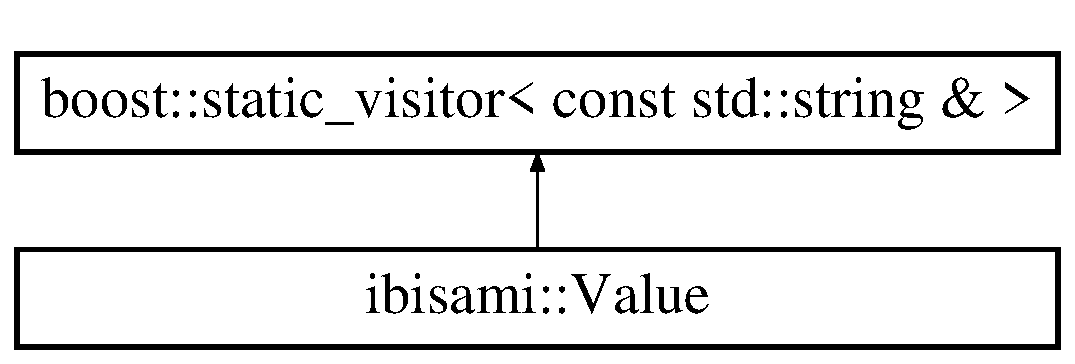
\includegraphics[height=2.000000cm]{structibisami_1_1_value}
\end{center}
\end{figure}
\subsection*{Public Member Functions}
\begin{DoxyCompactItemize}
\item 
const std\+::string \& \hyperlink{structibisami_1_1_value_ac3233a56bec33b072bc669cb617a0f4b}{operator()} (const \hyperlink{structibisami_1_1_param_tree}{ibisami\+::\+Param\+Tree} \&param\+\_\+tree) const 
\item 
const std\+::string \& \hyperlink{structibisami_1_1_value_aa74e1ca6fe4abdbe048cc58deacbefed}{operator()} (const std\+::string \&val\+\_\+str) const 
\end{DoxyCompactItemize}


\subsection{Detailed Description}
Used to access a {\itshape leaf} node. 

Definition at line 56 of file amimodel.\+h.



\subsection{Member Function Documentation}
\hypertarget{structibisami_1_1_value_ac3233a56bec33b072bc669cb617a0f4b}{}\index{ibisami\+::\+Value@{ibisami\+::\+Value}!operator()@{operator()}}
\index{operator()@{operator()}!ibisami\+::\+Value@{ibisami\+::\+Value}}
\subsubsection[{operator()}]{\setlength{\rightskip}{0pt plus 5cm}const std\+::string\& ibisami\+::\+Value\+::operator() (
\begin{DoxyParamCaption}
\item[{const {\bf ibisami\+::\+Param\+Tree} \&}]{param\+\_\+tree}
\end{DoxyParamCaption}
) const\hspace{0.3cm}{\ttfamily [inline]}}\label{structibisami_1_1_value_ac3233a56bec33b072bc669cb617a0f4b}


Definition at line 57 of file amimodel.\+h.

\hypertarget{structibisami_1_1_value_aa74e1ca6fe4abdbe048cc58deacbefed}{}\index{ibisami\+::\+Value@{ibisami\+::\+Value}!operator()@{operator()}}
\index{operator()@{operator()}!ibisami\+::\+Value@{ibisami\+::\+Value}}
\subsubsection[{operator()}]{\setlength{\rightskip}{0pt plus 5cm}const std\+::string\& ibisami\+::\+Value\+::operator() (
\begin{DoxyParamCaption}
\item[{const std\+::string \&}]{val\+\_\+str}
\end{DoxyParamCaption}
) const\hspace{0.3cm}{\ttfamily [inline]}}\label{structibisami_1_1_value_aa74e1ca6fe4abdbe048cc58deacbefed}


Definition at line 58 of file amimodel.\+h.



The documentation for this struct was generated from the following file\+:\begin{DoxyCompactItemize}
\item 
ibisami/include/\hyperlink{amimodel_8h}{amimodel.\+h}\end{DoxyCompactItemize}

\chapter{File Documentation}
\hypertarget{example__tx_8cpp}{}\section{example/example\+\_\+tx.cpp File Reference}
\label{example__tx_8cpp}\index{example/example\+\_\+tx.\+cpp@{example/example\+\_\+tx.\+cpp}}


Example of using ibisami to build a Tx model.  


{\ttfamily \#include $<$string$>$}\\*
{\ttfamily \#include $<$vector$>$}\\*
{\ttfamily \#include \char`\"{}include/ami\+\_\+tx.\+h\char`\"{}}\\*
\subsection*{Classes}
\begin{DoxyCompactItemize}
\item 
class \hyperlink{class_my_tx}{My\+Tx}
\begin{DoxyCompactList}\small\item\em An example device specific Tx model implementation. \end{DoxyCompactList}\end{DoxyCompactItemize}
\subsection*{Macros}
\begin{DoxyCompactItemize}
\item 
\#define \hyperlink{example__tx_8cpp_af1850df0d59f876e56124608d292faad}{T\+A\+P\+\_\+\+S\+C\+A\+L\+E}~0.\+047
\end{DoxyCompactItemize}
\subsection*{Variables}
\begin{DoxyCompactItemize}
\item 
\hyperlink{class_my_tx}{My\+Tx} \hyperlink{example__tx_8cpp_a7477fa3c6e307f34f7d51829b16bb839}{my\+\_\+tx}
\item 
\hyperlink{class_a_m_i_model}{A\+M\+I\+Model} $\ast$ \hyperlink{example__tx_8cpp_aa0c4a4f61a9cc689992be1759eb7041a}{ami\+\_\+model} = \&\hyperlink{example__tx_8cpp_a7477fa3c6e307f34f7d51829b16bb839}{my\+\_\+tx}
\begin{DoxyCompactList}\small\item\em The pointer required by the A\+P\+I implementation. \end{DoxyCompactList}\end{DoxyCompactItemize}


\subsection{Detailed Description}
Example of using ibisami to build a Tx model. 

Original author\+: David Banas ~\newline
 Original date\+: May 8, 2015

Copyright (c) 2015 David Banas; all rights reserved World wide. 

\subsection{Macro Definition Documentation}
\hypertarget{example__tx_8cpp_af1850df0d59f876e56124608d292faad}{}\index{example\+\_\+tx.\+cpp@{example\+\_\+tx.\+cpp}!T\+A\+P\+\_\+\+S\+C\+A\+L\+E@{T\+A\+P\+\_\+\+S\+C\+A\+L\+E}}
\index{T\+A\+P\+\_\+\+S\+C\+A\+L\+E@{T\+A\+P\+\_\+\+S\+C\+A\+L\+E}!example\+\_\+tx.\+cpp@{example\+\_\+tx.\+cpp}}
\subsubsection[{T\+A\+P\+\_\+\+S\+C\+A\+L\+E}]{\setlength{\rightskip}{0pt plus 5cm}\#define T\+A\+P\+\_\+\+S\+C\+A\+L\+E~0.\+047}\label{example__tx_8cpp_af1850df0d59f876e56124608d292faad}


Definition at line 10 of file example\+\_\+tx.\+cpp.



\subsection{Variable Documentation}
\hypertarget{example__tx_8cpp_aa0c4a4f61a9cc689992be1759eb7041a}{}\index{example\+\_\+tx.\+cpp@{example\+\_\+tx.\+cpp}!ami\+\_\+model@{ami\+\_\+model}}
\index{ami\+\_\+model@{ami\+\_\+model}!example\+\_\+tx.\+cpp@{example\+\_\+tx.\+cpp}}
\subsubsection[{ami\+\_\+model}]{\setlength{\rightskip}{0pt plus 5cm}{\bf A\+M\+I\+Model}$\ast$ ami\+\_\+model = \&{\bf my\+\_\+tx}}\label{example__tx_8cpp_aa0c4a4f61a9cc689992be1759eb7041a}


The pointer required by the A\+P\+I implementation. 

Defined in our device-\/specific source code file. 

Definition at line 70 of file example\+\_\+tx.\+cpp.

\hypertarget{example__tx_8cpp_a7477fa3c6e307f34f7d51829b16bb839}{}\index{example\+\_\+tx.\+cpp@{example\+\_\+tx.\+cpp}!my\+\_\+tx@{my\+\_\+tx}}
\index{my\+\_\+tx@{my\+\_\+tx}!example\+\_\+tx.\+cpp@{example\+\_\+tx.\+cpp}}
\subsubsection[{my\+\_\+tx}]{\setlength{\rightskip}{0pt plus 5cm} {\bf My\+Tx}  my\+\_\+tx}\label{example__tx_8cpp_a7477fa3c6e307f34f7d51829b16bb839}

\hypertarget{test_8py}{}\section{example/test.py File Reference}
\label{test_8py}\index{example/test.\+py@{example/test.\+py}}
\subsection*{Namespaces}
\begin{DoxyCompactItemize}
\item 
 \hyperlink{namespacetest}{test}
\end{DoxyCompactItemize}
\subsection*{Variables}
\begin{DoxyCompactItemize}
\item 
string \hyperlink{namespacetest_a80f837d5da2fad005c3ba8151a77ff62}{test.\+g\+D\+L\+L\+Name} = \textquotesingle{}./example\+\_\+tx\+\_\+x86\+\_\+amd64.\+so\textquotesingle{}
\item 
tuple \hyperlink{namespacetest_a353d01c7c783fd0d6d6287c760facb41}{test.\+the\+\_\+model} = ami.\+A\+M\+I\+Model(g\+D\+L\+L\+Name)
\item 
tuple \hyperlink{namespacetest_aebc7edb91e3546a519a0954d1fc0130d}{test.\+init\+\_\+data} = ami.\+A\+M\+I\+Model\+Initializer(\{\textquotesingle{}root\+\_\+name\textquotesingle{}\+: \char`\"{}example\+Tx\char`\"{}\})
\end{DoxyCompactItemize}

\hypertarget{ami__tx_8h}{}\section{include/ami\+\_\+tx.h File Reference}
\label{ami__tx_8h}\index{include/ami\+\_\+tx.\+h@{include/ami\+\_\+tx.\+h}}


Interface to \hyperlink{class_ami_tx}{Ami\+Tx} class.  


{\ttfamily \#include $<$string$>$}\\*
{\ttfamily \#include $<$vector$>$}\\*
{\ttfamily \#include \char`\"{}include/amimodel.\+h\char`\"{}}\\*
{\ttfamily \#include \char`\"{}include/digital\+\_\+filter.\+h\char`\"{}}\\*
\subsection*{Classes}
\begin{DoxyCompactItemize}
\item 
class \hyperlink{class_ami_tx}{Ami\+Tx}
\begin{DoxyCompactList}\small\item\em A generic I\+B\+I\+S-\/\+A\+M\+I Tx model implementation. \end{DoxyCompactList}\end{DoxyCompactItemize}


\subsection{Detailed Description}
Interface to \hyperlink{class_ami_tx}{Ami\+Tx} class. 

Original author\+: David Banas ~\newline
 Original date\+: May 6, 2015

Copyright (c) 2015 David Banas; all rights reserved World wide. 
\hypertarget{amimodel_8h}{}\section{include/amimodel.h File Reference}
\label{amimodel_8h}\index{include/amimodel.\+h@{include/amimodel.\+h}}


Interface to \hyperlink{class_a_m_i_model}{A\+M\+I\+Model} class.  


{\ttfamily \#include $<$boost/spirit/include/qi.\+hpp$>$}\\*
{\ttfamily \#include $<$boost/spirit/include/qi\+\_\+omit.\+hpp$>$}\\*
{\ttfamily \#include $<$boost/spirit/include/phoenix\+\_\+core.\+hpp$>$}\\*
{\ttfamily \#include $<$boost/spirit/include/phoenix\+\_\+fusion.\+hpp$>$}\\*
{\ttfamily \#include $<$boost/spirit/include/phoenix\+\_\+operator.\+hpp$>$}\\*
{\ttfamily \#include $<$boost/spirit/include/phoenix\+\_\+stl.\+hpp$>$}\\*
{\ttfamily \#include $<$boost/variant.\+hpp$>$}\\*
{\ttfamily \#include $<$boost/fusion/include/adapt\+\_\+struct.\+hpp$>$}\\*
{\ttfamily \#include $<$fstream$>$}\\*
{\ttfamily \#include $<$string$>$}\\*
{\ttfamily \#include $<$vector$>$}\\*
{\ttfamily \#include $<$utility$>$}\\*
\subsection*{Classes}
\begin{DoxyCompactItemize}
\item 
struct \hyperlink{structibisami_1_1_param_tree}{ibisami\+::\+Param\+Tree}
\begin{DoxyCompactList}\small\item\em The parameter tree definition. \end{DoxyCompactList}\item 
struct \hyperlink{structibisami_1_1_value}{ibisami\+::\+Value}
\begin{DoxyCompactList}\small\item\em Used to access a {\itshape leaf} node. \end{DoxyCompactList}\item 
struct \hyperlink{structibisami_1_1_node}{ibisami\+::\+Node}
\begin{DoxyCompactList}\small\item\em Used to access a {\itshape branch} node. \end{DoxyCompactList}\item 
class \hyperlink{class_a_m_i_model}{A\+M\+I\+Model}
\begin{DoxyCompactList}\small\item\em Abstract class providing the base functionality required by all I\+B\+I\+S-\/\+A\+M\+I models. \end{DoxyCompactList}\end{DoxyCompactItemize}
\subsection*{Namespaces}
\begin{DoxyCompactItemize}
\item 
 \hyperlink{namespaceibisami}{ibisami}
\begin{DoxyCompactList}\small\item\em Used to protect several complex custom types from potential name collisions. \end{DoxyCompactList}\end{DoxyCompactItemize}
\subsection*{Macros}
\begin{DoxyCompactItemize}
\item 
\#define \hyperlink{amimodel_8h_ab851168a21246c759c23a126c192360f}{P\+R\+B\+S\+\_\+\+L\+E\+N}~7
\end{DoxyCompactItemize}
\subsection*{Typedefs}
\begin{DoxyCompactItemize}
\item 
typedef boost\+::variant$<$ boost\+::recursive\+\_\+wrapper$<$ Param\+Tree $>$, std\+::string $>$ \hyperlink{namespaceibisami_a56481565abb44593a678738f57c04109}{ibisami\+::\+Param\+Node}
\item 
typedef std\+::pair$<$ bool, std\+::string $>$ \hyperlink{amimodel_8h_a5fbe8bcd249e7070ded2dadafa23ec1f}{Parse\+Res}
\end{DoxyCompactItemize}
\subsection*{Functions}
\begin{DoxyCompactItemize}
\item 
\hyperlink{amimodel_8h_a3b6210648aa742440c6393c5c5ff64b3}{B\+O\+O\+S\+T\+\_\+\+F\+U\+S\+I\+O\+N\+\_\+\+A\+D\+A\+P\+T\+\_\+\+S\+T\+R\+U\+C\+T} (\hyperlink{structibisami_1_1_param_tree}{ibisami\+::\+Param\+Tree},(std\+::string, name)(std\+::vector$<$ \hyperlink{namespaceibisami_a56481565abb44593a678738f57c04109}{ibisami\+::\+Param\+Node} $>$, children)) namespace ibisami
\end{DoxyCompactItemize}


\subsection{Detailed Description}
Interface to \hyperlink{class_a_m_i_model}{A\+M\+I\+Model} class. 

Original author\+: David Banas ~\newline
 Original date\+: May 1, 2015

Copyright (c) 2015 David Banas; all rights reserved World wide.

This abstract class provides the common base for all A\+M\+I models. 

\subsection{Macro Definition Documentation}
\hypertarget{amimodel_8h_ab851168a21246c759c23a126c192360f}{}\index{amimodel.\+h@{amimodel.\+h}!P\+R\+B\+S\+\_\+\+L\+E\+N@{P\+R\+B\+S\+\_\+\+L\+E\+N}}
\index{P\+R\+B\+S\+\_\+\+L\+E\+N@{P\+R\+B\+S\+\_\+\+L\+E\+N}!amimodel.\+h@{amimodel.\+h}}
\subsubsection[{P\+R\+B\+S\+\_\+\+L\+E\+N}]{\setlength{\rightskip}{0pt plus 5cm}\#define P\+R\+B\+S\+\_\+\+L\+E\+N~7}\label{amimodel_8h_ab851168a21246c759c23a126c192360f}


Definition at line 28 of file amimodel.\+h.



\subsection{Typedef Documentation}
\hypertarget{amimodel_8h_a5fbe8bcd249e7070ded2dadafa23ec1f}{}\index{amimodel.\+h@{amimodel.\+h}!Parse\+Res@{Parse\+Res}}
\index{Parse\+Res@{Parse\+Res}!amimodel.\+h@{amimodel.\+h}}
\subsubsection[{Parse\+Res}]{\setlength{\rightskip}{0pt plus 5cm}typedef std\+::pair$<$bool, std\+::string$>$ {\bf Parse\+Res}}\label{amimodel_8h_a5fbe8bcd249e7070ded2dadafa23ec1f}


Definition at line 118 of file amimodel.\+h.



\subsection{Function Documentation}
\hypertarget{amimodel_8h_a3b6210648aa742440c6393c5c5ff64b3}{}\index{amimodel.\+h@{amimodel.\+h}!B\+O\+O\+S\+T\+\_\+\+F\+U\+S\+I\+O\+N\+\_\+\+A\+D\+A\+P\+T\+\_\+\+S\+T\+R\+U\+C\+T@{B\+O\+O\+S\+T\+\_\+\+F\+U\+S\+I\+O\+N\+\_\+\+A\+D\+A\+P\+T\+\_\+\+S\+T\+R\+U\+C\+T}}
\index{B\+O\+O\+S\+T\+\_\+\+F\+U\+S\+I\+O\+N\+\_\+\+A\+D\+A\+P\+T\+\_\+\+S\+T\+R\+U\+C\+T@{B\+O\+O\+S\+T\+\_\+\+F\+U\+S\+I\+O\+N\+\_\+\+A\+D\+A\+P\+T\+\_\+\+S\+T\+R\+U\+C\+T}!amimodel.\+h@{amimodel.\+h}}
\subsubsection[{B\+O\+O\+S\+T\+\_\+\+F\+U\+S\+I\+O\+N\+\_\+\+A\+D\+A\+P\+T\+\_\+\+S\+T\+R\+U\+C\+T}]{\setlength{\rightskip}{0pt plus 5cm}B\+O\+O\+S\+T\+\_\+\+F\+U\+S\+I\+O\+N\+\_\+\+A\+D\+A\+P\+T\+\_\+\+S\+T\+R\+U\+C\+T (
\begin{DoxyParamCaption}
\item[{{\bf ibisami\+::\+Param\+Tree}}]{, }
\item[{(std\+::string, name)(std\+::vector$<$ {\bf ibisami\+::\+Param\+Node} $>$, children)}]{}
\end{DoxyParamCaption}
)}\label{amimodel_8h_a3b6210648aa742440c6393c5c5ff64b3}


Definition at line 76 of file amimodel.\+h.


\hypertarget{digital__filter_8h}{}\section{include/digital\+\_\+filter.h File Reference}
\label{digital__filter_8h}\index{include/digital\+\_\+filter.\+h@{include/digital\+\_\+filter.\+h}}


Interface to \hyperlink{class_digital_filter}{Digital\+Filter} class.  


{\ttfamily \#include $<$vector$>$}\\*
\subsection*{Classes}
\begin{DoxyCompactItemize}
\item 
class \hyperlink{class_digital_filter}{Digital\+Filter}
\begin{DoxyCompactList}\small\item\em A generic digital filter implementation, using \char`\"{}\+Direct Form 2\char`\"{} processing. \end{DoxyCompactList}\end{DoxyCompactItemize}


\subsection{Detailed Description}
Interface to \hyperlink{class_digital_filter}{Digital\+Filter} class. 

Original author\+: David Banas ~\newline
 Original date\+: May 7, 2015

Copyright (c) 2015 David Banas; all rights reserved World wide.

This class provides a generic digital filter. 
\hypertarget{main_8dox}{}\section{main.\+dox File Reference}
\label{main_8dox}\index{main.\+dox@{main.\+dox}}

\hypertarget{_r_e_a_d_m_e_8md}{}\section{R\+E\+A\+D\+M\+E.\+md File Reference}
\label{_r_e_a_d_m_e_8md}\index{R\+E\+A\+D\+M\+E.\+md@{R\+E\+A\+D\+M\+E.\+md}}

\hypertarget{ami__tx_8cpp}{}\section{ibisami/src/ami\+\_\+tx.cpp File Reference}
\label{ami__tx_8cpp}\index{ibisami/src/ami\+\_\+tx.\+cpp@{ibisami/src/ami\+\_\+tx.\+cpp}}


Implementation of \hyperlink{class_ami_tx}{Ami\+Tx} class.  


{\ttfamily \#include $<$string$>$}\\*
{\ttfamily \#include \char`\"{}include/ami\+\_\+tx.\+h\char`\"{}}\\*


\subsection{Detailed Description}
Implementation of \hyperlink{class_ami_tx}{Ami\+Tx} class. 

Original author\+: David Banas ~\newline
 Original date\+: May 7, 2015

Copyright (c) 2015 David Banas; all rights reserved World wide. 
\hypertarget{amimodel_8cpp}{}\section{ibisami/src/amimodel.cpp File Reference}
\label{amimodel_8cpp}\index{ibisami/src/amimodel.\+cpp@{ibisami/src/amimodel.\+cpp}}


Implementation of \hyperlink{class_a_m_i_model}{A\+M\+I\+Model} class.  


{\ttfamily \#include $<$string$>$}\\*
{\ttfamily \#include $<$utility$>$}\\*
{\ttfamily \#include $<$vector$>$}\\*
{\ttfamily \#include \char`\"{}include/amimodel.\+h\char`\"{}}\\*


\subsection{Detailed Description}
Implementation of \hyperlink{class_a_m_i_model}{A\+M\+I\+Model} class. 

Original author\+: David Banas~\newline
 Original date\+: May 2, 2015

Copyright (c) 2015 David Banas; all rights reserved World wide. 
\hypertarget{digital__filter_8cpp}{}\section{src/digital\+\_\+filter.cpp File Reference}
\label{digital__filter_8cpp}\index{src/digital\+\_\+filter.\+cpp@{src/digital\+\_\+filter.\+cpp}}


Implementation of \hyperlink{class_digital_filter}{Digital\+Filter} class.  


{\ttfamily \#include $<$vector$>$}\\*
{\ttfamily \#include \char`\"{}include/digital\+\_\+filter.\+h\char`\"{}}\\*


\subsection{Detailed Description}
Implementation of \hyperlink{class_digital_filter}{Digital\+Filter} class. 

Original author\+: David Banas ~\newline
 Original date\+: May 7, 2015

Copyright (c) 2015 David Banas; all rights reserved World wide. 
\hypertarget{ibisami__api_8cpp}{}\section{src/ibisami\+\_\+api.cpp File Reference}
\label{ibisami__api_8cpp}\index{src/ibisami\+\_\+api.\+cpp@{src/ibisami\+\_\+api.\+cpp}}


Provides I\+B\+I\+S-\/\+A\+M\+I A\+P\+I and necessary bootstrapping.  


{\ttfamily \#include $<$stdexcept$>$}\\*
{\ttfamily \#include $<$string$>$}\\*
{\ttfamily \#include \char`\"{}include/amimodel.\+h\char`\"{}}\\*
\subsection*{Classes}
\begin{DoxyCompactItemize}
\item 
struct \hyperlink{struct_ami_pointers}{Ami\+Pointers}
\begin{DoxyCompactList}\small\item\em Holds the pointers, which we pass back to the \hyperlink{ibisami__api_8cpp_a2518d31187e06bed6023ec23657faab9}{A\+M\+I\+\_\+\+Init()} caller. \end{DoxyCompactList}\end{DoxyCompactItemize}
\subsection*{Macros}
\begin{DoxyCompactItemize}
\item 
\#define \hyperlink{ibisami__api_8cpp_a1ca888bd091694c05472e1b91df1a97b}{D\+L\+L\+\_\+\+E\+X\+P\+O\+R\+T}
\end{DoxyCompactItemize}
\subsection*{Functions}
\begin{DoxyCompactItemize}
\item 
\hyperlink{ibisami__api_8cpp_a1ca888bd091694c05472e1b91df1a97b}{D\+L\+L\+\_\+\+E\+X\+P\+O\+R\+T} long \hyperlink{ibisami__api_8cpp_a2518d31187e06bed6023ec23657faab9}{A\+M\+I\+\_\+\+Init} (double $\ast$impulse\+\_\+matrix, long number\+\_\+of\+\_\+rows, long aggressors, double sample\+\_\+interval, double bit\+\_\+time, char $\ast$A\+M\+I\+\_\+parameters\+\_\+in, char $\ast$$\ast$A\+M\+I\+\_\+parameters\+\_\+out, void $\ast$$\ast$A\+M\+I\+\_\+memory\+\_\+handle, char $\ast$$\ast$msg)
\begin{DoxyCompactList}\small\item\em I\+B\+I\+S-\/\+A\+M\+I model initialization and impulse response processing. (Required) \end{DoxyCompactList}\item 
\hyperlink{ibisami__api_8cpp_a1ca888bd091694c05472e1b91df1a97b}{D\+L\+L\+\_\+\+E\+X\+P\+O\+R\+T} long \hyperlink{ibisami__api_8cpp_a5290351461f5a1fdf0e8cf061b306b2a}{A\+M\+I\+\_\+\+Close} (void $\ast$A\+M\+I\+\_\+memory)
\begin{DoxyCompactList}\small\item\em Clean-\/up. (Required) \end{DoxyCompactList}\end{DoxyCompactItemize}
\subsection*{Variables}
\begin{DoxyCompactItemize}
\item 
\hyperlink{class_a_m_i_model}{A\+M\+I\+Model} $\ast$ \hyperlink{ibisami__api_8cpp_aa0c4a4f61a9cc689992be1759eb7041a}{ami\+\_\+model}
\begin{DoxyCompactList}\small\item\em Defined in our device-\/specific source code file. \end{DoxyCompactList}\end{DoxyCompactItemize}


\subsection{Detailed Description}
Provides I\+B\+I\+S-\/\+A\+M\+I A\+P\+I and necessary bootstrapping. 

Original author\+: David Banas ~\newline
 Original date\+: April 29, 2015

Copyright (c) 2015 David Banas; all rights reserved World wide.

Provides the A\+P\+I (application programming interface) to the $\ast$.S\+O (shared object) or $\ast$.D\+L\+L (dynamically linked library) file.

Note\+: The required A\+P\+I for a I\+B\+I\+S-\/\+A\+M\+I model is defined by the I\+B\+I\+S standard, which is available here\+: \href{http://www.eda.org/ibis/}{\tt http\+://www.\+eda.\+org/ibis/} 

\subsection{Macro Definition Documentation}
\hypertarget{ibisami__api_8cpp_a1ca888bd091694c05472e1b91df1a97b}{}\index{ibisami\+\_\+api.\+cpp@{ibisami\+\_\+api.\+cpp}!D\+L\+L\+\_\+\+E\+X\+P\+O\+R\+T@{D\+L\+L\+\_\+\+E\+X\+P\+O\+R\+T}}
\index{D\+L\+L\+\_\+\+E\+X\+P\+O\+R\+T@{D\+L\+L\+\_\+\+E\+X\+P\+O\+R\+T}!ibisami\+\_\+api.\+cpp@{ibisami\+\_\+api.\+cpp}}
\subsubsection[{D\+L\+L\+\_\+\+E\+X\+P\+O\+R\+T}]{\setlength{\rightskip}{0pt plus 5cm}\#define D\+L\+L\+\_\+\+E\+X\+P\+O\+R\+T}\label{ibisami__api_8cpp_a1ca888bd091694c05472e1b91df1a97b}


Definition at line 37 of file ibisami\+\_\+api.\+cpp.



\subsection{Function Documentation}
\hypertarget{ibisami__api_8cpp_a5290351461f5a1fdf0e8cf061b306b2a}{}\index{ibisami\+\_\+api.\+cpp@{ibisami\+\_\+api.\+cpp}!A\+M\+I\+\_\+\+Close@{A\+M\+I\+\_\+\+Close}}
\index{A\+M\+I\+\_\+\+Close@{A\+M\+I\+\_\+\+Close}!ibisami\+\_\+api.\+cpp@{ibisami\+\_\+api.\+cpp}}
\subsubsection[{A\+M\+I\+\_\+\+Close}]{\setlength{\rightskip}{0pt plus 5cm}{\bf D\+L\+L\+\_\+\+E\+X\+P\+O\+R\+T} long A\+M\+I\+\_\+\+Close (
\begin{DoxyParamCaption}
\item[{void $\ast$}]{A\+M\+I\+\_\+memory}
\end{DoxyParamCaption}
)}\label{ibisami__api_8cpp_a5290351461f5a1fdf0e8cf061b306b2a}


Clean-\/up. (Required) 


\begin{DoxyParams}{Parameters}
{\em A\+M\+I\+\_\+memory} & A pointer to the model memory structure. \\
\hline
\end{DoxyParams}
\begin{DoxyReturn}{Returns}
\textquotesingle{}1\textquotesingle{} 
\end{DoxyReturn}


Definition at line 133 of file ibisami\+\_\+api.\+cpp.

\hypertarget{ibisami__api_8cpp_a2518d31187e06bed6023ec23657faab9}{}\index{ibisami\+\_\+api.\+cpp@{ibisami\+\_\+api.\+cpp}!A\+M\+I\+\_\+\+Init@{A\+M\+I\+\_\+\+Init}}
\index{A\+M\+I\+\_\+\+Init@{A\+M\+I\+\_\+\+Init}!ibisami\+\_\+api.\+cpp@{ibisami\+\_\+api.\+cpp}}
\subsubsection[{A\+M\+I\+\_\+\+Init}]{\setlength{\rightskip}{0pt plus 5cm}{\bf D\+L\+L\+\_\+\+E\+X\+P\+O\+R\+T} long A\+M\+I\+\_\+\+Init (
\begin{DoxyParamCaption}
\item[{double $\ast$}]{impulse\+\_\+matrix, }
\item[{long}]{number\+\_\+of\+\_\+rows, }
\item[{long}]{aggressors, }
\item[{double}]{sample\+\_\+interval, }
\item[{double}]{bit\+\_\+time, }
\item[{char $\ast$}]{A\+M\+I\+\_\+parameters\+\_\+in, }
\item[{char $\ast$$\ast$}]{A\+M\+I\+\_\+parameters\+\_\+out, }
\item[{void $\ast$$\ast$}]{A\+M\+I\+\_\+memory\+\_\+handle, }
\item[{char $\ast$$\ast$}]{msg}
\end{DoxyParamCaption}
)}\label{ibisami__api_8cpp_a2518d31187e06bed6023ec23657faab9}


I\+B\+I\+S-\/\+A\+M\+I model initialization and impulse response processing. (Required) 


\begin{DoxyParams}{Parameters}
{\em impulse\+\_\+matrix} & A matrix of doubles containing, at least, the impulse response to be processed (i.\+e. -\/ the victim), in place. \\
\hline
{\em number\+\_\+of\+\_\+rows} & The length of all impulse responses provided (victim and aggressors). \\
\hline
{\em aggressors} & The number of aggressors included in impulse\+\_\+matrix. \\
\hline
{\em sample\+\_\+interval} & The time interval between adjacent elements of the vectors contained in impulse\+\_\+matrix. \\
\hline
{\em bit\+\_\+time} & The unit interval. \\
\hline
{\em A\+M\+I\+\_\+parameters\+\_\+in} & A pointer to a char array containing the input A\+M\+I parameter string. \\
\hline
{\em A\+M\+I\+\_\+parameters\+\_\+out} & A handle to be updated with the pointer to the output A\+M\+I parameter string. \\
\hline
{\em A\+M\+I\+\_\+memory\+\_\+handle} & A handle to be updated with the pointer to the model memory structure. \\
\hline
{\em msg} & A handle to be updated with the pointer to the message being returned by the model. \\
\hline
\end{DoxyParams}
\begin{DoxyReturn}{Returns}
\textquotesingle{}1\textquotesingle{} for success, \textquotesingle{}0\textquotesingle{} for failure. 
\end{DoxyReturn}


Definition at line 53 of file ibisami\+\_\+api.\+cpp.



\subsection{Variable Documentation}
\hypertarget{ibisami__api_8cpp_aa0c4a4f61a9cc689992be1759eb7041a}{}\index{ibisami\+\_\+api.\+cpp@{ibisami\+\_\+api.\+cpp}!ami\+\_\+model@{ami\+\_\+model}}
\index{ami\+\_\+model@{ami\+\_\+model}!ibisami\+\_\+api.\+cpp@{ibisami\+\_\+api.\+cpp}}
\subsubsection[{ami\+\_\+model}]{\setlength{\rightskip}{0pt plus 5cm}{\bf A\+M\+I\+Model}$\ast$ ami\+\_\+model}\label{ibisami__api_8cpp_aa0c4a4f61a9cc689992be1759eb7041a}


Defined in our device-\/specific source code file. 

Defined in our device-\/specific source code file. 

Definition at line 144 of file example\+\_\+rx.\+cpp.


%--- End generated contents ---

% Index
\backmatter
\newpage
\phantomsection
\clearemptydoublepage
\addcontentsline{toc}{chapter}{Index}
\printindex

\end{document}
